

%\documentclass[10pt,a4paper]{article}
\documentclass[runningheads]{llncs}

\usepackage[utf8]{inputenc}
\usepackage{amsmath,amsfonts,amssymb}
\usepackage{thmtools}
%\usepackage{amsthm}
\usepackage{thm-restate}

\usepackage{hyperref}
\usepackage[capitalize, noabbrev]{cleveref}
\usepackage{graphicx}
\usepackage{color}
\usepackage{enumerate}
\usepackage{caption}
\usepackage{subcaption}

\usepackage{tikz,tikzsymbols}
\usetikzlibrary{shapes,patterns,positioning}
\usetikzlibrary{arrows,decorations.markings}
\usetikzlibrary{calc}

                  
%%%%%%%%%%%%%%%%%%%%%%%%%%%%%%%%%%%%%%%%%%%%%%
%%  Lasse: macros
%%%%%%%%%%%%%%%%%%%%%%%%%%%%%%%%%%%%%%%%%%%%%%
\newcommand{\R}{\mathbb{R}}
\newcommand{\N}{\mathbb{N}}
\newcommand{\Z}{\mathbb{Z}}
\newcommand{\set}[1]{\{ #1 \}}
\newcommand{\fromto}[2]{\set{#1, \ldots, #2}}

\newcommand{\comment}[1]{\textcolor{red}{(L: #1)}}

\newcommand{\bigO}{\mathcal{O}}
\newcommand{\dotunion}{\mathbin{\dot{\cup}}}
\DeclareMathOperator{\opt}{OPT}

%%%%%%%%%%%%%%%%%%%%%%%%%%%%%%%%%%%%%%%%%%%%%%
%%  GJW: macros
%%%%%%%%%%%%%%%%%%%%%%%%%%%%%%%%%%%%%%%%%%%%%%
\DeclareMathOperator{\ntp}{\text{\sf ntp}}
\newcommand{\xxxNTP}{{\sc N-TreePack}}
\newcommand{\greedy}{\text{\sf Greedy}}


%%%%%%%%%%%%%%%%%%%%%%%%%%%%%%%%%%%%%%%%%%%%%%%%%%%%%%%%%%%%%%%%%%%%%%%%%%
%%%%%%%%%%%%%%%%%%%%%%%%%%%%%%%%%%%%%%%%%%%%%%%%%%%%%%%%%%%%%%%%%%%%%%%%%%
%%%%%%%%%%%%%%%%%%%%%%%%%%%%%%%%%%%%%%%%%%%%%%%%%%%%%%%%%%%%%%%%%%%%%%%%%%
%%%%%%%%%%%%%%%%%%%%%%%%%%%%%%%%%%%%%%%%%%%%%%%%%%%%%%%%%%%%%%%%%%%%%%%%%%
\sloppy
\begin{document}

\title{Non-preemptive tree packing}
\titlerunning{Non-preemptive tree packing}

\author{Stefan Lendl\inst{1} \and
Gerhard Woeginger\inst{2} \and
Lasse Wulf\inst{3}}

\authorrunning{S. Lendl, G. Woeginger, and L. Wulf}
\institute{Department of Operations and Information Systems, University of Graz, Austria 
\email{stefan.lendl@uni-graz.at}\\
\and Department of Computer Science, RWTH Aachen, Germany 
\email{woeginger@algo.rwth-aachen.de}\\
\and Institute of Discrete Mathematics, Graz University of Technology, Austria\\
\email{wulf@math.tugraz.at}
}
%
\maketitle 

\begin{abstract}
An instance of the non-preemptive tree packing problem consists of an undirected graph $G=(V,E)$ 
together with a weight $w(e)$ for every edge $e\in E$.
The goal is to activate every edge $e$ for some time interval of length $w(e)$, such that the 
activated edges form a connected spanning subgraph of $G$ for the longest possible overall time.

We derive a variety of results on this problem.
The problem is strongly NP-hard even on graphs of treewidth~$2$, and it does not allow a polynomial
time approximation scheme (unless P=NP).
Furthermore, we discuss the performance of a simple greedy algorithm, and we construct and analyze
a number of parametrized and exact algorithms.
\end{abstract}


%%%%%%%%%%%%%%%%%%%%%%%%%%%%%%%%%%%%%%%%%%%%%%%%%%%%%%%%%%%%%%%%%%%%%%%%%
%%%%%%%%%%%%%%%%%%%%%%%%%%%%%%%%%%%%%%%%%%%%%%%%%%%%%%%%%%%%%%%%%%%%%%%%%
\section{Introduction}
%%%%%%%%%%%%%%%%%%%%%%%%%%%%%%%%%%%%%%%%%%%%%%%%%%%%%%%%%%%%%%%%%%%%%%%%
\paragraph{The tree packing problem of Nash-Williams.}
For a given undirected connected graph $G=(V,E)$ and a weight function $w:E\to\N$,
Nash-Williams \cite{Nash-Williams1961} considered the following optimization problem:
%%%%%%%%%%%%%%%%%%%%%%%
\begin{align}
\text{maximize}~~ &\sum\left\{x_T:\,\text{$T$ is a spanning tree} \right\} 
\label{eq:NW.1} \\[0.5ex]
\text{such that}~~&\sum\left\{x_T:\,e\in T\right\}\le w(e)\qquad\text{for every $e\in E$}
\label{eq:NW.2} \\[0.5ex]
                 &x\ge0,~\text{integral}
\label{eq:NW.3} 
\end{align}
%%%%%%%%%%%%%%%%%%%%%%%
Nash-Williams \cite{Nash-Williams1961} derives a min-max relation for problem
\eqref{eq:NW.1}--\eqref{eq:NW.3} that connects it to certain cut conditions.
Building on these results, Cunningham \cite{Cunningham1985} constructs a polynomial time 
algorithm for the problem by reducing it to a polynomial number of maximum flow problems.

Problem \eqref{eq:NW.1}--\eqref{eq:NW.3} may also be interpreted as a scheduling problem:
Every edge $e\in E$ is a resource that can be activated for a total of $w(e)$ time units.
The objective now is to activate the edges in a such way that the graph remains connected 
for the longest possible overall time. 
Under this interpretation, the variable $x_T$ indicates the number of time units in which
the spanning tree $T$ is used in the activation schedule.
Figure~\ref{fig:example} contains a simple illustrating example on the three-vertex cycle.
There are three spanning trees (that each consist of two edges), and an optimal schedule 
uses each of these spanning trees for exactly one time unit.
It is easy to see that in every optimal schedule, one of the three edges will be active 
during the first and the third time slot and will be in-active during the second time slot;
in the language of scheduling, we say that the execution of that edge is preempted 
at time $1$ and afterwards resumed at time $2$.
(In the schedule shown in Figure~\ref{fig:example}, edge $e_3$ is the preempted edge.)

%%%%%%%%%%%%%%%%%%%%%%%%%%%%%%%%%%%%%%%%%
\begin{figure}[tbh]
\bigskip
\begin{center}
%%%%%%%%%%%%%%%%
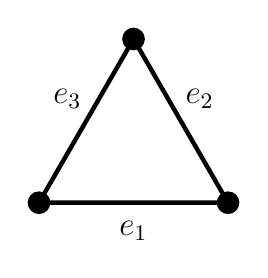
\begin{tikzpicture}[scale=1.20]
\coordinate (p1) at (-1,0);
\coordinate (p2) at ( 1,0);
\coordinate (p3) at ( 0,1.732);

\foreach \x in {1,2,3} \fill (p\x) circle (0.12);
\draw[ultra thick] (p1)--(p2)--(p3)--(p1);
\node[] at  ( 0.0,-0.3) {\large $e_1$};
\node[] at  ( 0.7, 1.1) {\large $e_2$};
\node[] at  (-0.7, 1.1) {\large $e_3$};
\end{tikzpicture}
%%%%%%%%%%%%%%%%
\qquad\qquad\qquad
%%%%%%%%%%%%%%%%

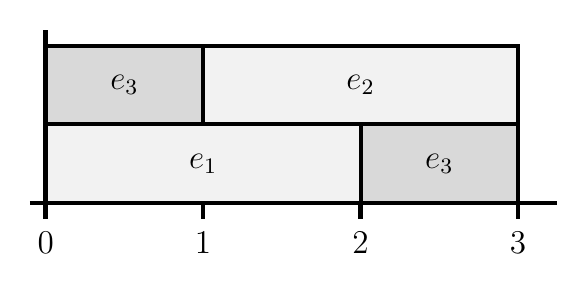
\begin{tikzpicture}[scale=1.00]
\draw[ultra thick] (-0.2,0)--(6.5,0);
\draw[ultra thick] (0,-0.2)--(0,2.2);

\node[] at  (0,-0.5) {\large $0$};
\draw[ultra thick] (2,-0.2)--(2,0);
\draw[ultra thick] (4,-0.2)--(4,0);
\draw[ultra thick] (6,-0.2)--(6,0);
\node[] at  (2,-0.5) {\large $1$};
\node[] at  (4,-0.5) {\large $2$};
\node[] at  (6,-0.5) {\large $3$};

\draw[fill=gray,fill opacity=0.1,draw=black,line width=1.5pt,text opacity=1.0]
       (0,0) rectangle (4,1) node[pos=.5] {\large $e_1$};
\draw[fill=gray,fill opacity=0.3,draw=black,line width=1.5pt,text opacity=1.0]
       (4,0) rectangle (6,1) node[pos=.5] {\large $e_3$};

\draw[fill=gray,fill opacity=0.3,draw=black,line width=1.5pt,text opacity=1.0]
       (0,1) rectangle (2,2) node[pos=.5] {\large $e_3$};
\draw[fill=gray,fill opacity=0.1,draw=black,line width=1.5pt,text opacity=1.0]
       (2,1) rectangle (6,2) node[pos=.5] {\large $e_2$};

\end{tikzpicture}
%%%%%%%%%%%%%%%%
\end{center}
\caption{The three edges in the graph on the left hand side have weights $w(e_1)=w(e_2)=w(e_3)=2$.
The schedule on the right hand side keeps the graph connected for a total of three time units.}
\label{fig:example}
\end{figure}
%%%%%%%%%%%%%%%%%%%%%%%%%%%%%%%%%%%%%%%%%

%%%%%%%%%%%%%%%%%%%%%%%%%%%%%%%%%%%%%%%%%
\paragraph{The non-preemptive version of tree packing.}
We consider a non-preemptive version of the above tree packing problem,
where the execution of edges must not be preempted: 
Every edge $e$ is activated at some time point $\tau(e)$ chosen by the scheduler, and then 
remains active without interruption during the full time interval $[\tau(e),\,\tau(e)+w(e)]$.
The objective is again to activate the edges in a such way that the graph
remains connected for the longest possible overall time.
The resulting combinatorial optimization problem is called \emph{non-preemptive tree packing}
({\xxxNTP} for short), and the optimal objective value for a graph $G=(V,E)$ with edge 
weights $w:E\to\N$ will be denoted $\ntp(G,w)$.

In the example in Figure~\ref{fig:example}, every reasonable non-preemptive
schedule will either activate two of the edges at time~$0$, or activate the three
edges respectively at times $0,1,2$.
As there is no way of keeping the graph connected for more than two time units, 
the optimal objective value is $\ntp(G,w)=2$.

%%%%%%%%%%%%%%%%%%%%%%%%%%%%%%%%%%%%%%%%%
\paragraph{Contributions of this paper.}
We analyze the computational complexity and the approximability of non-preemptive 
tree packing, and we also provide some parametrized and exact algorithms for it.
The complexity results are devastating:
\begin{itemize}
\item {\xxxNTP} is strongly NP-hard, even on complete bipartite graphs $K_{2,n}$.
\item {\xxxNTP} is strongly NP-hard, even on graphs of bandwidth~$2$.
\end{itemize}
Since complete bipartite graphs $K_{2,n}$ are series-parallel and since graphs of 
bandwidth~$2$ are outerplanar, our results yield strong NP-hardness for essentially 
all natural subclasses of graphs with treewidth~$2$.
As edges of zero-weight are irrelevant for the objective value of {\xxxNTP}, NP-hardness 
immediately propagates from graphs to supergraphs; hence our results also imply 
strong NP-hardness for all the standard families of specially structured graphs, 
like planar graphs, bipartite graphs, interval graphs, cographs, etc.
The only notable exception is the class of trees, on which {\xxxNTP} is 
straightforward to solve and uninteresting.

With respect to polynomial time approximation, we introduce a simple greedy algorithm.
This greedy algorithm has a worst case guarantee of $n-1$ on $n$-vertex graphs,
and on cactus graphs it always succeeds in finding an optimal solution.
We also show that for every non-cactus graph $G$, there exist edge weights $w$ so
that for the input $(G,w)$ the greedy algorithm fails to find an optimal solution.
We show by means of a gap-reduction that (unless P$=$NP) problem {\xxxNTP} does not
allow a polynomial time approximation algorithm with worst case ratio strictly below $7/6$;
this of course excludes the existence of a PTAS.

Finally, we derive a number of FPT-results in the area of parametrized complexity.
The special case of {\xxxNTP} where both the treewidth and the maximum edge weight are 
bounded by a constant $k$ allows an FPT-algorithm whose running time is linear in $|E|$.
(The case where only the treedwidth is bounded and the case where only the maximum 
edge weight is bounded are NP-hard, and hence do not belong to FPT.)
Furthermore we design an exact algorithm for {\xxxNTP} whose (exponential) 
running time is bounded by $|E|!\cdot\text{poly}(|E|)$.

%%%%%%%%%%%%%%%%%%%%%%%%%%%%%%%%%%%%%%%%%
\paragraph{Organization of the paper.}
Section~\ref{sec:notation} provides central definitions and summarizes the notation.
Section~\ref{sec:hardness} contains the NP-hardness results, and 
Section~\ref{sec:inapprox} contains the in-approximability result.
Section~\ref{sec:greedy} discusses the greedy algorithm, 
Section~\ref{sec:parameterized} states some parametrized and exact algorithms for {\xxxNTP}, and
Section~\ref{sec:conclusion} concludes the paper with some discussion.


%%%%%%%%%%%%%%%%%%%%%%%%%%%%%%%%%%%%%%%%%%%%%%%%%%%%%%%%%%%%%%%%%%%%%%%%%
%%%%%%%%%%%%%%%%%%%%%%%%%%%%%%%%%%%%%%%%%%%%%%%%%%%%%%%%%%%%%%%%%%%%%%%%%
\section{Definitions and Notations}
\label{sec:notation}
%%%%%%%%%%%%%%%%%%%%%%%%%%%%%%%%%%%%%%%%%%%%%%%%%%%%%%%%%%%%%%%%%%%%%%%%%
We write $\N_0 := \N \cup \set{0}$ for the set of nonnegative integers. 
For $a\le b$, the term $[a,b]$ denotes the \emph{time slot} starting at $a$ and ending at $b$. 
For $i\ge1$, the time slot $[i-1,i]$ is often called the $i$-th time slot.
All graphs in this paper are undirected, simple, and without loops.

An instance for problem {\xxxNTP} is a weighted graph $(G,w)$, where $G=(V,E)$ and $w:E\to\N$. 
A \emph{schedule} for instance $(G,w)$ is a map $\sigma:E\to\N_0$, that maps each edge $e$ to its activation time $\sigma(e)$;
For a schedule $\sigma$ and an edge $e$, we denote the \emph{activity interval of $e$} by $[\sigma(e),\sigma(e)+w(e)]$. 
For $i\in\{1,2,\ldots\}$, we let $E^\sigma_i:= \set{e\in E:~ \sigma(e)+1 \le i
\le \sigma(e)+w(e)}$ denote 
the set of edges that are active in the $i$-th time slot, and we let $G^\sigma_i:= (V, E^\sigma_i)$ denote 
the graph on vertex set $V$ and all edges, which are active in the $i$-th time slot. 
Finally, we define the \emph{objective value} $\ntp(\sigma)$ of schedule $\sigma$ as the number of time 
slots $[i-1,i]$ for which $G^\sigma_i$ is connected. If a schedule $\sigma$ has maximal objective value $\ntp(\sigma) = T$ among all possible schedules, we often assume that $G^\sigma_t$ is connected if and only if $t \in \fromto{1}{T}$. It is easy to see that this can be assumed without loss of generality. When the schedule $\sigma$ is clear from the context, we often simply write $E_i$ and $G_i$ instead of 
$E^\sigma_i$ and $G^\sigma_i$. 

We make use of the following graph-theoretic concepts and notations: 
Let $G=(V,E)$ be a graph. We sometimes write $V(G):=V$ and $E(G):=E$. 
For $V'\subseteq V$, the corresponding \emph{edge cut} $\delta(V')$ is the set of edges with
one endpoint in $V'$ and one endpoint in $V-V'$. 
For $v\in V$, we let $\delta(v) := \delta(\set{v})$. 
We denote by $G[V']$ the \emph{induced subgraph} on $V'$. 
By removing the vertex $v$ from $G$, we obtain the graph $G-v=G[V-\set{v}]$. 
Similarily, for $E'\subseteq E$ and $e\in E$ we have $G-E'=(V,E-E')$ and $G-e=G-\set{e}$.
For all other graph-theoretic concepts used in the paper, we refer the reader to the
text book by West \cite{WestBook}.


%%%%%%%%%%%%%%%%%%%%%%%%%%%%%%%%%%%%%%%%%%%%%%%%%%%%%%%%%%%%%%%%%%%%%%%%%
%%%%%%%%%%%%%%%%%%%%%%%%%%%%%%%%%%%%%%%%%%%%%%%%%%%%%%%%%%%%%%%%%%%%%%%%%
\section{NP-Hardness}
\label{sec:hardness}
%%%%%%%%%%%%%%%%%%%%%%%%%%%%%%%%%%%%%%%%%%%%%%%%%%%%%%%%%%%%%%%%%%%%%%%%%
In this section, we establish the NP-hardness of problem {\xxxNTP} for certain families of
highly restricted instances. 
This is done by reducing from the strongly NP-hard \textsc{3-Partition} problem;
see Garey \& Johnson \cite{garey1979computers}. 
%%%%%%%%%%%%%%%%%
\begin{quote}
Problem \textsc{3-Partition}: 
\\
\textbf{Instance:} Positive integers $a_1,\ldots,a_{3n}$ with sum $\sum_{i=1}^{3n}a_i=nQ$ that satisfy 
$Q/4<a_i<Q/2$ for all $i$.
\\
\textbf{Question}: Is there a partition of these $3n$ numbers into $n$ into triplets, such that in 
every triplet the three numbers sum up to $Q$?  
\end{quote}
%%%%%%%%%%%%%%%%%
In the following, we show that problem {\xxxNTP} is strongly NP-hard both for series-parallel graph 
(Theorem~\ref{thm:hardness_complete_bipartite}) and for graphs of bandwith~2 (Theorem~\ref{thm:hardness_bandwidth}). 

%%%%%%%%%%%%%%%%%
\begin{theorem}
\label{thm:hardness_complete_bipartite}
Problem {\xxxNTP} is strongly NP-hard, even on complete bipartite graphs $K_{2,n}$.
\end{theorem}
%%%%%%%%%%%%%%%%%
\begin{proof}
Let $a_1,\ldots,a_{3n}$ be an instance of \textsc{3-Partition} as defined above. 
Let $\beta := nQ + n - 1$. 
We construct an instance of {\xxxNTP} on the complete bipartite graph $K_{2,4n-1}$ with bipartition
$\set{s, t}$ and $\set{x_1, \ldots, x_{n-1}, y_1, \ldots, y_{3n}}$. 
For $i\in\{1, \dots,n-1\}$, we set $w(\set{s,x_i}):= i(Q + 1)$ and $w(\set{x_i,t}):=(n - i)(Q + 1)$. 
For $i\in\{1,\dots,3n\}$, we set $w(\set{s,y_i}):= a_i$ and $w(\set{y_i,t}):= \beta$. 

We claim that the constructed instance of {\xxxNTP} possesses a schedule with objective value $\beta$, 
if and only if the underlying \textsc{3-Partition} instance has answer YES.
(Only if): Assume that for the constructed {\xxxNTP} instance there exists a schedule $\sigma$ with objective value $\beta$. 
Note that for every $i \in \{1,\dots,n-1\}$, we have $w(\set{s,x_i}) + w(\set{x_i,t}) = \beta + 1$. 
Hence the sum of all the edge weights in the graph is $(n-1)(\beta + 1) + 3n\beta + (\beta - n + 1) = 4\beta n$. 
As every spanning tree for $K_{2, 4n-1}$ has $4n$ edges, each of the connected graphs $G_1,\dots,G_\beta$ 
must have exactly $4n$ edges (and must actually be a spanning tree). 
Now consider some vertex $x_i$ with $i\in\{1,\dots,n-1\}$. 
Since $w(\set{s,x_i}) + w(\set{x_i,t})=\beta+1$, there is exactly one $k\in\fromto{1}{\beta}$ so 
that the edge set $E_k$ contains both edges incident to vertex $x_i$. 
It is easy to see that either $k=i(Q+1)$ or $k=(n-i)(Q+1)$ holds, and we say that this value $k$ 
is associated with vertex $x_i$.
If some value $k$ is associated with two distinct vertices $x_i$ and $x_j$, then $G_k$ contains 
a cycle; a contradiction.
We conclude that each of the values $k\in\set{Q+1,2(Q+1),\ldots,(n-1)(Q+1)}$ is assosciated with
exactly one of the vertices $x_1,\ldots,x_{n-1}$.
This means that for the corresponding time slots $[k-1,k]$, vertex $s$ is connected to vertex $t$
via the two edges that are incident to the associated vertex $x_i$.
The remaining $\beta-n+1$ time slots form $n$ (maximal) intervals each of length $Q$.
It is easily verified that during each such interval exactly three vertices $y_i$, $y_j$, $y_{\ell}$
ensure the connection between $s$ and $t$, and that the weights of the three edges $\{s,y_i\}$,
$\{s,y_j\}$, $\{s,y_{\ell}\}$ satisfy $a_i+a_j+a_{\ell}=Q$.
Hence the corresponding triplets form a solution for the \textsc{3-Partition} instance.

(If) Vice versa, if the \textsc{3-Partition} instance has a solution, then it is easy to see that there exists a schedule $\sigma$
with objective value $\beta$. The schedule has the same properties as explained in the (only if) direction of this proof.
\qed
\end{proof}

%%%%%%%%%%%%%%%%%
\begin{theorem}
\label{thm:hardness_bandwidth}
Problem {\xxxNTP} is strongly NP-hard, even on graphs of bandwidth~$2$.
\end{theorem}
%%%%%%%%%%%%%%%%%
\begin{proof}
Let $a_1,\ldots,a_{3n}$ be an instance of \textsc{3-Partition} as defined above.
We construct an instance of {\xxxNTP} as follows.
The graph $G$ has $4n+1$ vertices $u_0,\ldots,u_n$ and $v_1,\ldots,v_{3n}$.
We will sometimes denote vertex $u_k$ also by the name $v_{k-n}$, for $1\le k\le n+1$;
in particular we use $u_n=v_0$ and $u_{n-1}=v_{-1}$.
\begin{itemize}
\item 
For $k=0,\ldots,n-1$,   the edge $\{u_k, u_{k+1}\}$ receives weight $w(\{u_k, u_{k+1}\}) = 2(n-k-1)Q$.
\item
For $k=0,\ldots,n-2$,   the edge $\{u_k, u_{k+2}\}$ receives weight $w(\{u_k, u_{k+2}\})=2(k+1)Q$.
\item 
For $k=1,\ldots,3n$,    the edge $\{v_{k-1}, v_k\}$ has weight $w(\{v_{k-1}, v_k\})=a_k$.
\item
For $k=-1,\ldots,3n-2$, the edge $\{v_k, v_{k+2}\}$ has weight $w(\{v_k, v_{k+2}\})=\beta$.  
\end{itemize}
In the ordering $u_0,u_1,\ldots,u_n,v_1,v_2,\ldots,v_{3n}$, every edge either connects two adjacent 
vertices or two vertices at distance~$2$. Hence, the constructed graph $G=(V,E)$ has bandwidth~$2$. 

We will study schedules $\sigma$ of objective value $\beta=(2n-1)Q$. 
As the sum of all edge weights in $G$ equals $\beta(|V|-1)$, each of the graphs 
$G^\sigma_1, \dots G^\sigma_\beta$ is a spanning tree.
We will discuss the behavior of $\sigma$ on the induced subgraph $H_i := G[\fromto{u_0}{u_i}]$ for $1\le i\le n$.
Since the only connections between $H_i$ and the rest of the graph are via the two vertices $u_{i-1}$ and $u_i$,
during any time slot $[t-1,t]$ with $1\le t\le\beta$, graph $H_i$ will consist of one or two connected components
under schedule $\sigma$.
If there is a single connected component, we say that $H_i$ is \emph{fully-connected} during the $t$-th time slot.
If there are two connected components (one containing vertex $u_{i-1}$, the other one containing 
vertex $u_i$), we say that $H_i$ is \emph{semi-connected} during the $t$-th time slot.
Note that if $H_i$ is semi-connected during the $t$-th time slot, then the edge $\{u_{i-1}, u_{i+1}\}$ must be 
active during that slot, as there are no other edges that would be able to connect the component containing 
$u_{i-1}$ to the rest of the graph.

The graph $H_1$ consists of the vertices $u_0$ and $u_1$ and of the edge $\{u_0, u_1\}$ of weight $(2n-2)Q$.
Suppose for the sake of contradiction that $H_1$ is neither fully-connnected during the first time slot
nor during the $\beta$-th time slot.
Then the edge $\{u_0, u_2\}$ (of value $2Q$) must be contained both in $E_1$ and in $E_{\beta}$, which is impossible.
By symmetry, we will henceforth assume that under schedule $\sigma$ the graph $G_1$ is fully-connnected 
during the $\beta$-th time slot.
This implies that $\{u_0, u_1\}$ is active during $[Q,\beta]$ and that $\{u_0, u_2\}$ is active during $[0,2Q]$.
For graph $H_i$ (with $1\le i\le n$) one can show by induction that $H_i$ is semi-connected
during the time intervals $[0,Q]$, $[2Q,3Q]$, \dots, $[(2i-2)Q,(2i-1)Q]$ and fully-connected at all
other moments in $[0,\beta]$.
The induction uses the following facts and observations on the two edges $\set{u_{i-2}, u_i}$ 
and $\set{u_{i-1},u_i}$ that are in $H_i$ but not in $H_{i-1}$:
\begin{itemize}
\item Graph $H_i$ is semi-connected during the first time slot:
By the inductive hypothesis we have $H_{i-1}$ semi-connected during the first time slot.
If $H_i$ would be fully-connected during the first time slot, we would get
$\sigma(\{u_{i-2}, u_i\}) = \sigma(\{u_{i-1}, u_i\})=0$. 
Since all involved edges have weight $w(e)>Q$, this yields a cycle at time $t=Q+1$ as the desired contradiction.
\item Since graph $H_{i-1}$ is semi-connected at time $0$, the edge $\{u_{i-2},u_i\}$ must be active at 
time $0$ and hence must be active during $[0,(2i-2)Q]$.
\item Graph $H_i$ must be fully-connnected during the $\beta$-th time slot:
Otherwise, $H_i$ is fully-connnected neither during the first time slot nor during the $\beta$-th time slot. 
Then the edge $\{u_{i-1},u_{i+1}\}$ would have to be active for $\beta$ time units.
\item Since $H_i$ is fully-connnected during the $\beta$-th time slot, the edge $\{u_{i-1},u_i\}$ must be 
active during the $\beta$-th time slot, and hence must be active during the interval $[(2i-1)Q,\beta]$.
\end{itemize}
The induction yields for $i=n$ that the induced subgraph $H_n$ is semi-connected during the time intervals 
$[0,Q]$, $[2Q,3Q]$, \dots, $[(2n-2)Q,(2n-1)Q]$ (that is, all the intervals of length $Q$ that start at an even multiple of $Q$)
and fully-connected during the time intervals $[Q,2Q]$, $[3Q,4Q]$, \dots, $[(2n-3)Q,(2n-2)Q]$ (that is, all the 
intervals of length $Q$ that start at an odd time multiple of $Q$).

Next, consider the subgraph $G'$ that is induced by the $3n+2$ vertices $v_{-1}=u_{n-1}$, $v_0=u_n$ and 
$v_1,\ldots,v_{3n}$.
As the edges $\{v_k, v_{k+2}\}$ with $k=-1,\ldots,3n-2$ all have value $\beta$, there is an active path $P_0$ 
through the vertices with even index during the full interval $[0,\beta]$ and there is an active 
path $P_1$ through the vertices with odd index during $[0, \beta]$.
By the above discussion, graph $H_n$ connects these two paths $P_0$ and $P_1$ to each other during the
time intervals $[Q,2Q]$, $[3Q,Q4]$, \dots, $[(2n-3)Q,(2n-2)Q]$.
The only way for connecting $P_0$ and $P_1$ to each other during the remaining time intervals 
$[0,Q]$, $[2Q,3Q]$, \dots, $[(2n-2)Q,(2n-1)Q]$ is by using the edges $\{v_{k-1},v_k\}$ with $k=1,\ldots,3n$ of 
weight $a_k$.
As this groups the numbers $a_1,\ldots,a_{3n}$ into $n$ groups with sum $Q$, we get a solution
for the instance of \textsc{3-Partition}.
Vice versa, if the \textsc{3-Partition} instance has a solution, then we can build a schedule $\sigma$
with all desired properties from it.
\end{proof}

%%%%%%%%%%%%%%%%%%%%%%%%%%%%%%%%%%%%%%%%%%%%%%%%%%%%%%%%%%%%%%%%%%%%%%%%%
%%%%%%%%%%%%%%%%%%%%%%%%%%%%%%%%%%%%%%%%%%%%%%%%%%%%%%%%%%%%%%%%%%%%%%%%%
\section{Hardness of Approximation}
\label{sec:inapprox}
%%%%%%%%%%%%%%%%%%%%%%%%%%%%%%%%%%%%%%%%%%%%%%%%%%%%%%%%%%%%%%%%%%%%%%%%%

In this section, we show that for problem {\xxxNTP} it is NP-hard to decide whether there exists a schedule of objective value at least 7. Our results imply that even if all edges have weights in $\fromto{1}{6}$, problem {\xxxNTP} is strongly NP-hard and  does not admit a polynomial time $\alpha$-approximation with $\alpha < 7/6$ (unless P$=$NP).
%We now show hardness even if the weights $w(e)$ are restricted. 
We reduce from the following version of the Hamilton cycle problem:

\begin{quote}

Problem \textsc{Hamilton'} 

\textbf{Instance:} A bipartite, 4-regular graph $H$, and an edge $\set{u, z}$ in $H$.

\textbf{Question:} Is there a Hamilton cycle which uses the edge $\set{u, z}$?

\end{quote}

There is a small technical complication: In the upcoming proof, we will require in one case that there exists a Hamilton cycle using the edge $\set{u,z}$, however, in another case we can only show that there exists a Hamilton path starting at vertex $u$. The following shows that we do not need to be concerned about the difference: An instance $(H, \set{u,z})$ of problem \textsc{Hamilton'}  is called \emph{hamilton-nice}, if $H$ either contains both a Hamilton cycle using the edge $\set{u,z}$ and a Hamilton path starting at vertex $u$, or contains none of the two.

\begin{restatable}{lemma}{hamiltonPrime}
\label{hamilton_cycle_lemma}
\mbox{\sc Hamilton'} is NP-complete, even when restricted to the set of hamilton-nice instances.
\end{restatable} 

This result is surely known, however, we were unable to find it in the literature. Using the fact that the Hamilton cycle problem is NP-complete on 3-regular, bipartite graphs, as proven by Akiyama, Nishizeki and Saito \cite{hamilton3regularBip}, the proof of \cref{hamilton_cycle_lemma} is an easy exercise (hence we omit it). We are now ready to describe the reduction from problem \textsc{Hamilton'} to problem {\xxxNTP}.

\paragraph{Description of the reduction.} Given an instance $(H, \set{u,z})$ of \textsc{Hamilton'}, we define the \emph{corresponding instance} of problem {\xxxNTP} to be the weighted graph $(G, w)$ described as follows: First, let $2k$ be the number of vertices of $H$. Let $U = \fromto{u_1}{u_k}$ and $Z = \fromto{z_1}{z_k}$ denote the two parts of the bipartition of $H$, such that $u = u_k$ and $z = z_k$. A sketch of the graph $G$ is depicted in \cref{fig:act-hamilton-cycle-a}. Informally speaking, $G$ is created from a copy of $H$, two additional vertices $x, y$, the edges $\set{x,y}$ and $\set{y, z_k}$ and for each $i = 1,\dots, k$ a gadget of type $L$ connecting $x$ with $u_i$, and for each $i = 1,\dots, k$ a gadget of type $R$ connecting $x$ with $z_i$. Formally, $G$ has the vertex set 
\[ V(G) = \set{x, y} \cup U \cup Z \cup \bigcup_{i=1}^k \fromto{v_{i1}}{v_{i4}} \cup \bigcup_{i=1}^k \set{v'_{i1}, v'_{i2}} \]
and the following edges and edge weights:
\begin{itemize}
\item For every edge $e \in E(H)$, the graph $G$ also contains $e$. We set $w(e) = 2$, if $e \neq \set{u_k, z_k}$ and $w(\set{u_k, z_k}) = 1$.
\item For every $i = 1,\dots,k$, the induced subgraph $G[\set{x, u_i, v_{i1}, v_{i2}, v_{i3}, v_{i4}}]$ is called the \emph{$i$-th gadget of type L} and has edges and edge weights as depicted in \cref{fig:act-hamilton-cycle-b}.
\item For every $i = 1,\dots,k$, the induced subgraph $G[\set{x, z_i, v'_{i1}, v'_{i2}}]$ is called the \emph{$i$-th gadget of type R} and has edges and edge weights as depicted in \cref{fig:act-hamilton-cycle-c}.
\item Finally, the two edges $\set{x,y}$ and $\set{y, z_k}$ have $w(\set{x,y}) = w(\set{y, z_k}) = 4$.
\end{itemize}
\begin{figure}[htpb]
     \centering
     \begin{subfigure}[b]{0.40\textwidth}
         \centering
         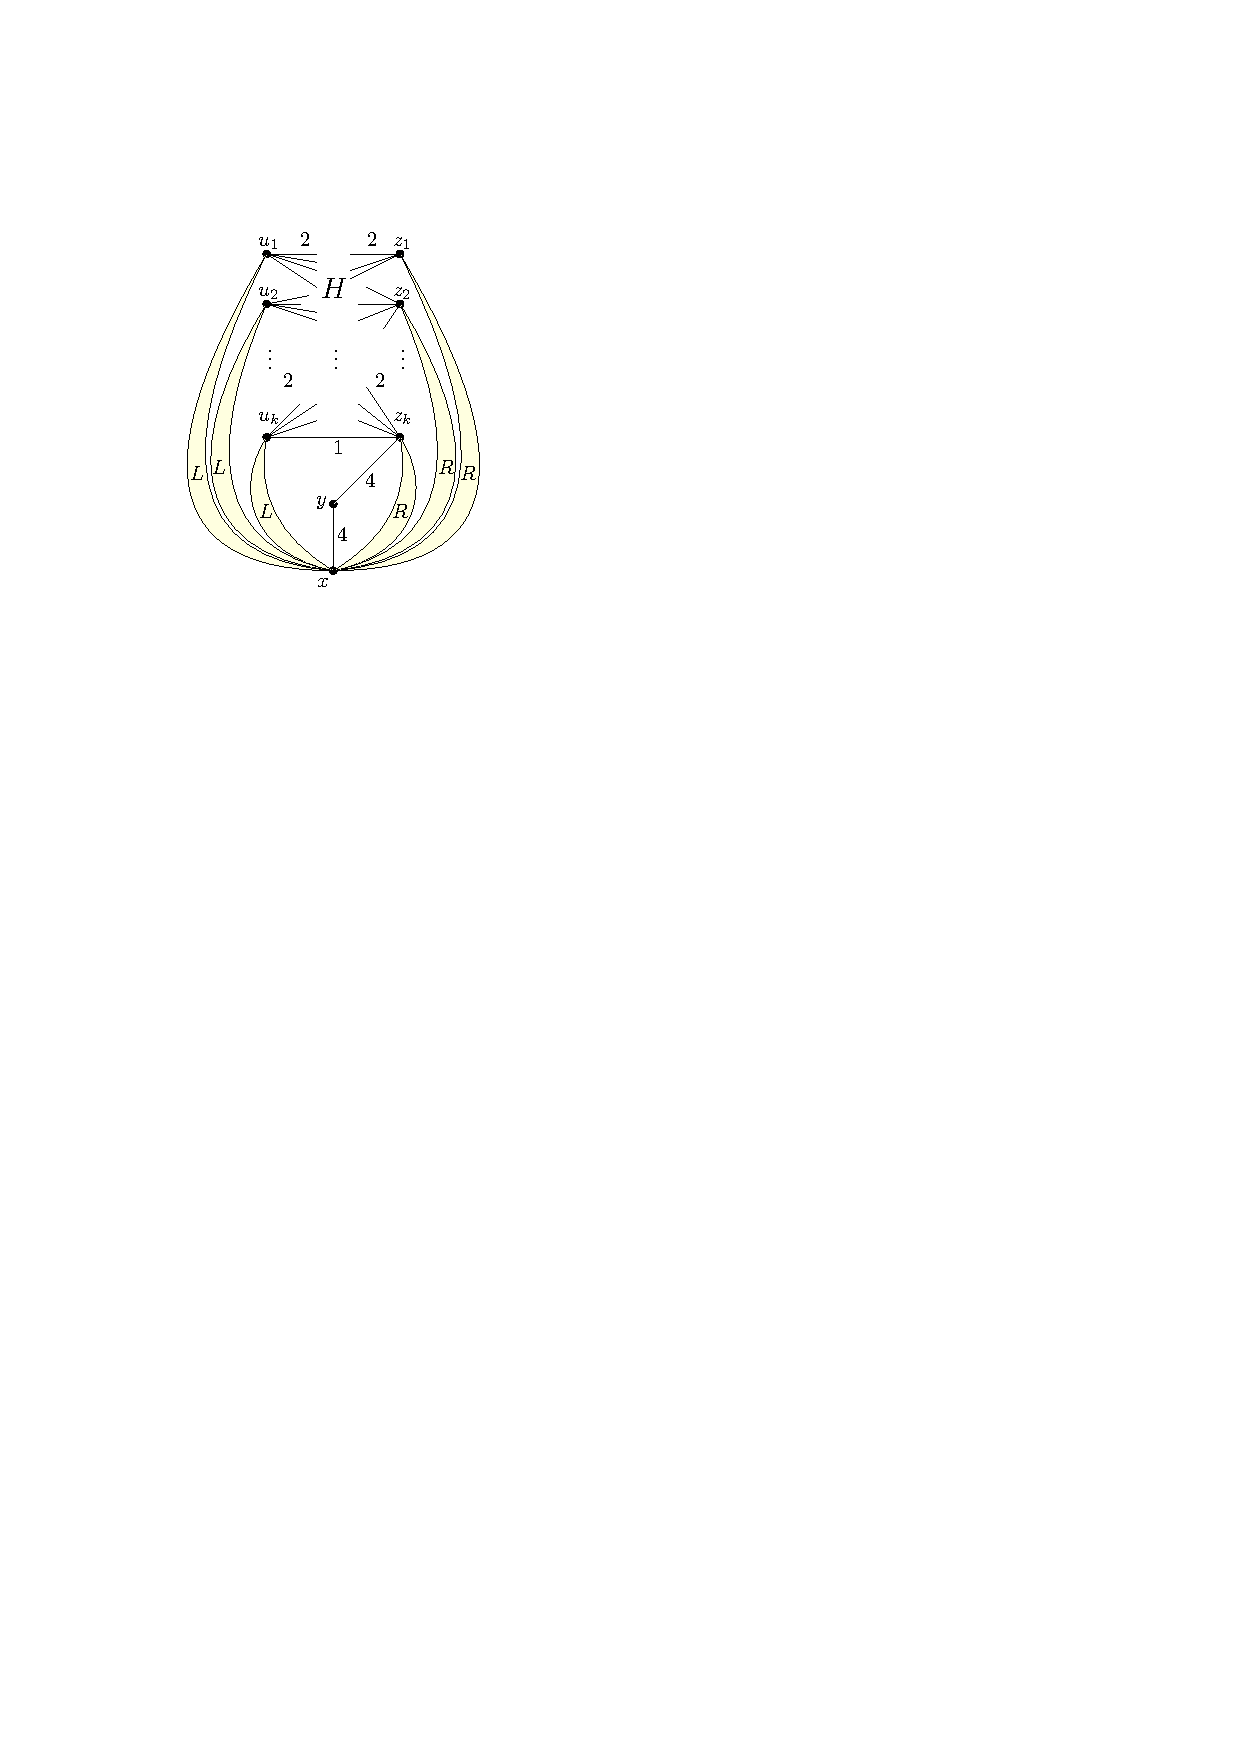
\includegraphics[scale=1]{img/act-hamilton-cycle-a}
         \subcaption{Reduction}
         \label{fig:act-hamilton-cycle-a}
     \end{subfigure}
     \hfill
     \begin{subfigure}[b]{0.32\textwidth}
         \centering
         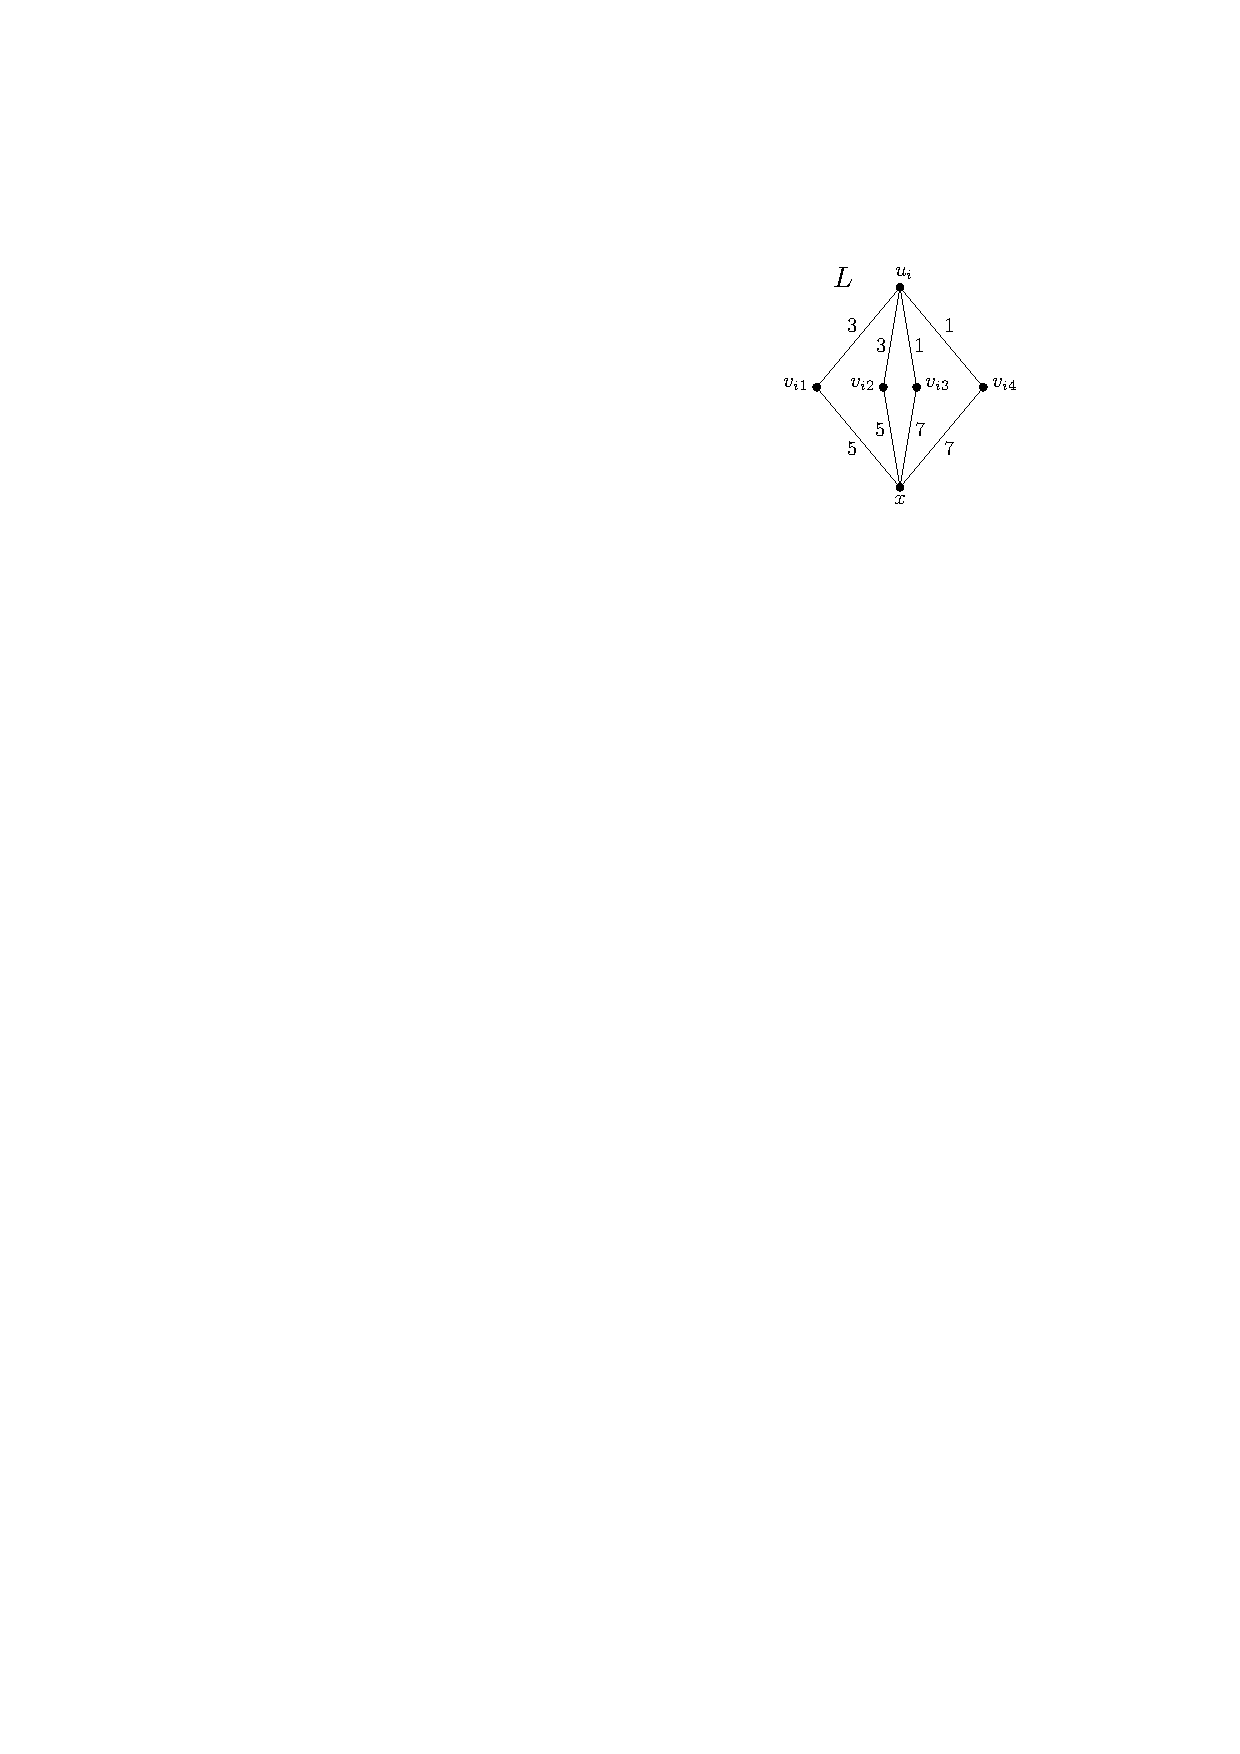
\includegraphics[scale=1]{img/act-hamilton-cycle-b-simplified}
         \subcaption{Gadget of type $L$}
         \label{fig:act-hamilton-cycle-b}
     \end{subfigure}
     \hfill
     \begin{subfigure}[b]{0.15\textwidth}
         \centering
         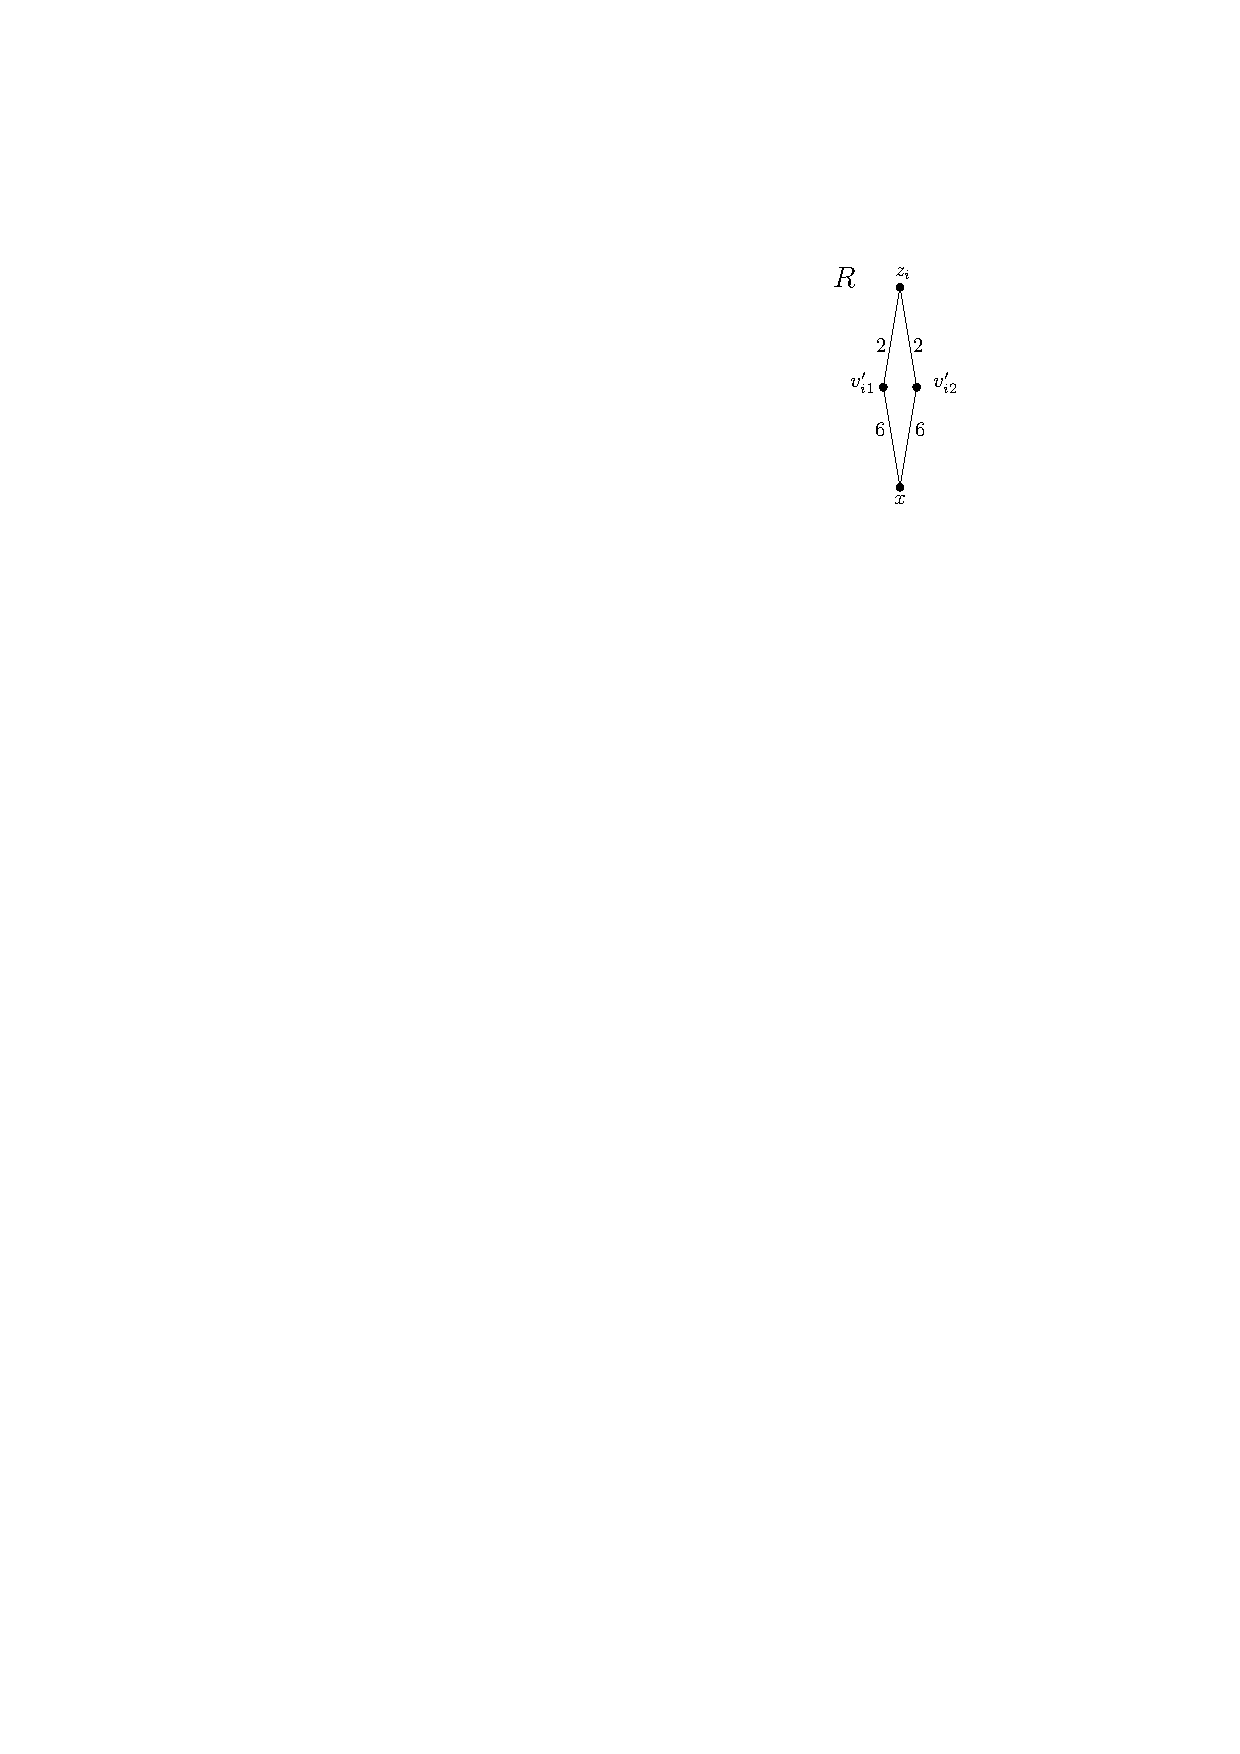
\includegraphics[scale=1]{img/act-hamilton-cycle-c}
         \subcaption{Gadget of type $R$}
         \label{fig:act-hamilton-cycle-c}
     \end{subfigure}
        \caption{Reduction \textsc{Hamilton'} $\rightarrow$ {\xxxNTP}.}
        \label{fig_act_hamilton_cycle}
\end{figure}

The main idea of the hardness proof is to prove that the gadgets impose restrictions in such a way, that in any schedule of objective value 7, the active edges during the 4th time slot form a Hamilton path (starting at vertex $u_k$) in $H$. Let $\sigma$ be some schedule for $(G, w)$ of objective value 7 and consider the $i$-th gadget of type $L$. Observe that during any time slot $[t-1, t]$ with $1 \leq t \leq 7$, the gagdet will consist of one or two connected components under schedule $\sigma$. If there is a single connected component, we say that this gadget is \emph{fully-connected} during the $t$-th time slot. If there are two connected components, we say that this gadget is \emph{semi-connected} during the $t$-th time slot. It is easy to see that $x$ and $u_i$ lie in different components in the latter case. In the same matter, during the $t$-th time slot, a gadget of type $R$ is either fully-connected or semi-connected with $x$ and $z_i$ in different components. Likewise, the induced subgraph $G[\set{x, y, z_k}]$ is either fully-connected, or semi-connected with $x$ and $z_k$ in different components.

\begin{lemma}
\label{lemma:gadgets_properties}
Let $(G, w)$ be the instance as described above. If there is a schedule of objective value 7 for $(G, w)$, then with respect to this schedule:
\begin{enumerate}[(i)]
\item A gadget of type $R$ is fully-connected during time slots 2 and 6, and semi-connected during each of the remaining five time slots 1, 3, 4, 5, and 7.
\item There exist distinct values $t_1, t_2 \in \set{1,2,4,6,7}$, such that a gadget of type $L$ is fully-connected during each of the four time slots $3,5,t_1$, and $t_2$, and semi-connected during each of the remaining three time slots.
\item The induced subgraph $G[\set{x, y, z_k}]$ is fully-connected during time slot 4, and semi-connected during each of the remaining six time slots 1, 2, 3, 5, 6, and 7.
\end{enumerate}
\end{lemma}
\begin{proof}
 Note that the sum of all edge weights in $G$ is $8k - 1 + 32k + 16k + 8 = 56k + 7 = 7(|V(G)| - 1)$. Therefore, each of $G_{1}, \ldots, G_{7}$ is a tree, and in particular acyclic. For the proof of (i), consider the vertex $v'_{i1}$ in the $i$-th gadget of type $R$. There is exactly one time slot $[t-1, t]$ during which both edges incident to $v'_{i1}$ are active, and we have $t = 2$ or $t = 6$. Analogously, there is exactly one time slot $[t'-1, t']$ during which both edges incident to $v'_{i2}$ are active, and we have $t' = 2$ or $t' = 6$. But if $t = t'$, then $G_t$ has a cycle; a contradiction. Therefore, $\set{t, t'} = \set{2, 6}$ and claim (i) follows. It is easily seen that the claims (ii) and (iii) can be proven in the same manner. 
\end{proof}

\begin{lemma}
\label{lemma:inapprox-if}
Let $(H, \set{u, z})$ be an instance of \textsc{Hamilton'}, and let $(G, w)$ be the corresponding {\xxxNTP} instance. If $H$ contains a Hamilton cycle using the edge $\set{u, z}$, then there is a schedule with objective value 7 for $(G, w)$.
\end{lemma}
\begin{proof}
Let $e_0 := \set{u, z} = \set{u_k, z_k}$. There is a Hamilton cycle $C$ using $e_0$. Then $H - E(C)$ is 2-regular, hence there exist pairwise disjoint matchings $M_1, \ldots, M_4$ such that $M_1 \dotunion M_2 = E(C)$ and $M_3 \dotunion M_4 = E(H)-E(C)$ and $e_0 \in M_1$. We describe a schedule $\sigma$ with objective value 7:
\begin{itemize}
\item All gagdets of type $R$ are fully-connected during time slots 2 and 6, and semi-connected otherwise.
\item All gadgets of type $L$ are fully-connected during time slots 1, 3, 5, and 7, and semi-connected otherwise.
\item The subgraph $G[\set{x, y, z_k}]$ is fully-connected during time slot 4, and semi-connected otherwise.
\item All edges $e \in M_1 - \set{e_0}$ have activity interval $[2, 4]$. The edge $e_0$ has activity interval $[2, 3]$.
\item All edges $e \in M_2$ have activity interval $[3, 5]$.
\item All edges $e \in M_3$ have activity interval $[0, 2]$.
\item All edges $e \in M_4$ have activity interval $[5, 7]$.
\end{itemize}
It is now easy to see that the active edges in $H$ form a matching of $H$ during the time slots 1,2,3,5,6, and 7, and form a Hamilton path of $H$ during the time slot 4. Indeed, all of the graphs $G^\sigma_1, \dots G^\sigma_7$. are connected, so $\sigma$ has objective value 7, as claimed.
\end{proof}

\begin{lemma}
\label{lemma:inapprox-only-if}
Let $(H, \set{\tilde{u}, \tilde{z}})$ be an instance of \textsc{Hamilton'}, and let $(G, w)$ be the corresponding {\xxxNTP} instance. If $(G, w)$ has a schedule of length 7, then $H$ contains a Hamilton path starting at vertex $\tilde{u}$.
\end{lemma}
\begin{proof}
 So assume there exists a schedule $\sigma$ of objective value 7. For a vertex $v \in U \cup Z$, and $t \in \fromto{1}{7}$, let $d_t(v) := |\delta(v) \cap E(H) \cap E_t|$ denote the number of incident edges of $v$, which are both in $E(H)$ and active during the $t$-th time slot. The strategy of the proof will be to repeatedly deduce some conditions for $d_t(v)$. Let $e_0 := \set{\tilde{u}, \tilde{z}} = \set{u_k, z_k}$.

First, recall \cref{lemma:gadgets_properties}. Consider a vertex $z \in Z$. We know that for each $t \in \set{1, 3, 5, 7}$ in the $t$-th time slot all gadgets of type $R$ and also $G[\set{x,y,z_k}]$ are semi-connected. This implies $d_1(z), d_3(z), d_5(z), d_7(z) \geq 1$.  Note that the four edges in $\delta(z) \cap E(H)$ each have weight at most 2 (in the case $z \neq z_k$ we have four times weight 2, and for $z = z_k$ we have three times weight 2, and $e_0$ has weight 1). So consider the process of arraging four intervals of length at most 2 in the interval $[0, 7]$ in such a way, that each of the time slots $[0,1], [2,3], [4,5], [6,7]$ is covered by at least one interval. Due to the properties of this process, one sees that the case $d_1(z) > 1$ or $d_7(z) > 1$ is actually impossible. Hence, $d_1(z) = d_7(z) = 1$. The same argument shows that $e_0 \not\in E_4$.

Next, consider the graph $G_1$ of active edges in time slot 1. We know that  $d_1(z) = 1$ for $z \in Z$. But this implies that the induced subgraph $G_1[U \cup Z]$ has $k$ connected components. Because $G_1$ is connected, and because all the gadgets of type $R$ and $G[\set{x, y, z_k}]$ are semi-connected during this time slot, this implies that every single gadget of type $L$ is actually fully-connected. The same argument holds for time slot 7. In total, together with \cref{lemma:gadgets_properties}, we have that a gadget of type $L$ is fully-connected during the $t$-th time slot, if and only if $t \in \set{1, 3, 5, 7}$. This in turn implies that for $u \in U$, one has $d_2(u), d_4(u), d_6(u) \geq 1$. The two facts $d_2(u) \geq 1$ and $d_6(u) \geq 1$ together imply $d_4(u) \leq 2$, due to the process described previously. Likewise, for $z \in Z$, the two facts $d_1(z) = 1$ and $d_7(z) = 1$ together imply $d_4(z) \leq 2$.

Finally, we claim $d_4(u_k) = 1$. In fact, $d_4(u_k) = 0$ is impossible, because gadgets of type $L$ are semi-connected during time slot 4. For the sake of contradiction, assume $d_4(u_k) > 1$. We know that $d_2(u_k) \geq 1, d_6(u_k) \geq 1$ and $e_0 \not\in E_4$ and $w(e_0) = 1$. So our assumption $d_4(u_k) > 1$ is only possible if $e_0 \in E_2$ or $e_0 \in E_6$. But for the vertex $z_k$, we also know $d_1(z_k), d_3(z_k), d_5(z_k), d_7(z_k) \geq 1$. This is a contradiction to $e_0 \in E_2 \cup E_6$, hence our assumption was wrong and $d_4(u_k) = 1$.

In summary, during time slot 4, all gadgets of type $L$ and $R$ are semi-connected. We also have $d_4(u) \leq 2$ for $u \in U$, and $d_4(z) \leq 2$ for $z \in Z$ and $d_4(u_k) = 1$. However, $G_4$ is connected. These facts together imply that the induced subgraph $G_4[U \cup Z]$ is a Hamilton path in $H$ starting at $u_k = \tilde{u}$.
\end{proof}

We remark, that one can make a small improvement, so that the graph $(G, w)$ actually only uses edges with weights in $\fromto{1}{6}$ instead of $\fromto{1}{7}$. Details are shown in \cref{appendix:small-weights-improvement}. In summary, combining \cref{hamilton_cycle_lemma,lemma:inapprox-only-if,lemma:inapprox-if}, we get:

\begin{theorem}
\label{th:small-weights}
Problem {\xxxNTP} is strongly NP-hard, even if all edges have weights in $\fromto{1}{6}$.
In particular, it is NP-hard to decide whether there exists a schedule with objective value at least~$7$.
\end{theorem}

\begin{corollary}
\label{coro:inapproximability}
Unless $P=NP$, problem {\xxxNTP} does not allow a polynomial time $\alpha$-approximation 
with $\alpha<7/6$.
\end{corollary}

%%%%%%%%%%%%%%%%%%%%%%%%%%%%%%%%%%%%%%%%%%%%%%%%%%%%%%%%%%%%%%%%%%%%%%%%%
%%%%%%%%%%%%%%%%%%%%%%%%%%%%%%%%%%%%%%%%%%%%%%%%%%%%%%%%%%%%%%%%%%%%%%%%%
\section{Small objective Values}
\label{sec:small-objective}
%%%%%%%%%%%%%%%%%%%%%%%%%%%%%%%%%%%%%%%%%%%%%%%%%%%%%%%%%%%%%%%%%%%%%%%%
In \cref{sec:inapprox}, we showed that it is NP-hard to decide whether a schedule of objective value at least 7 exists. In contrast, we show that it can be decided in polynomial time, whether a schedule of objective value at least 3 exists.


\begin{theorem}
Given an instance $(G, w)$ of {\xxxNTP} on $m$ edges, it can be decided in $\bigO(m^3)$ time, whether $\ntp(G, w) \geq 3$.
\end{theorem}
\begin{proof}
Let $G = (V, E)$. If we only want to know whether $\ntp(G, w) \geq 3$, then every edge of weight $w(e) > 3$ behaves just like an edge of weight $w(e) = 3$. Hence we assume $w(e) \in \set{1,2,3}$ for all edges. Let for $k = 1,2,3$ the edges of weight $k$ be denoted by $E'_k = \set{e \in E \mid w(e) = k}$. In a schedule of objective value 3, we can assume that an edge of weight 3 is scheduled during $[0, 3]$. We can also interpret an edge of length 2 as being a pair of two different edges of weight 1: One of these edges always gets scheduled in time slot $[1, 2]$, and for the other edge, the scheduler can choose whether to schedule it either during $[0, 1]$ or during $[2, 3]$. For $t = 1,2,3$, we consider the matroid of edges that can be scheduled during the $t$-th time slot. Formally, let $H_3$ be the graph resulting from $G$ after contracting the edge set $E'_3$, and let $H_{23}$ be the graph resulting from $G$ after contracting the edge set $E'_2 \cup E'_3$. Consider the matroids $\mathcal{F}_1 = \mathcal{F}_3 := \set{F \subseteq E'_1 \cup E'_2 \mid F \text{ is acyclic in }H_3}$ and $\mathcal{F}_2 := \set{F \subseteq E'_1 \mid F \text{ is acyclic in }H_{23}}$. By the properties of this construction, we have that $\ntp(G, w) \geq 3$ if and only if there exists $E'' \subseteq E'_1 \cup E'_2$ and a partition $P_1 \dotunion P_2 \dotunion P_3 = E''$ of $E''$, such that $P_i$ is a base of the matroid $\mathcal{F}_i$ for $i=1,2,3$. This can be checked using for example Edmond's matroid partitioning algorithm \cite{edmonds1965minimum} in $\bigO(m^3)$ time.

Using a similar argument, the question, whether $\ntp(G, w) \geq 2$ can easily be reduced to Nash-Williams tree packing problem. The question, whether $\ntp(G, w) \geq 1$ is trivial.
\end{proof}

%%%%%%%%%%%%%%%%%%%%%%%%%%%%%%%%%%%%%%%%%%%%%%%%%%%%%%%%%%%%%%%%%%%%%%%%%
%%%%%%%%%%%%%%%%%%%%%%%%%%%%%%%%%%%%%%%%%%%%%%%%%%%%%%%%%%%%%%%%%%%%%%%%%
\section{The greedy Algorithm}
\label{sec:greedy}
%%%%%%%%%%%%%%%%%%%%%%%%%%%%%%%%%%%%%%%%%%%%%%%%%%%%%%%%%%%%%%%%%%%%%%%%
We introduce a simple greedy algorithm that maintains connectivity by always
activating edges of the largest possible weight.
Formally, we let $E_i\subseteq E$ denote the set of edges that are active during
the $i$-th time slot $[i-1,\,i]$, and we let $F_i\subseteq E_i$ denote the set of
edges whose activity intervals end at time $i$.
Finally, we denote by $U_i=E-(E_1\cup E_2\cup\cdots E_i)$ the set of edges that
have not been used and activated before time $i$.

Now the {\greedy} algorithm starts its work by initializing 
$E_0:=\emptyset$, $F_0:=\emptyset$, and $U_0:=E$.
For $i\ge0$, the set $E_{i+1}$ for time slot $[i,\,i+1]$ is computed as follows.
If the graph $(V,E_i-F_i)$ is a tree, we set $E_{i+1}:=E_i$.
If the graph $(V,E_i-F_i)$ is a forest with $c$ components, we turn it into 
a tree by adding a maximum weight subset $A\subseteq U_i$ of cardinality $c-1$;
then we set $E_{i+1}:=(E_i-F_i)\cup A$.
In case no such set $A$ exists, the {\greedy} algorithm terminates.
(The set $A$ can be computed for instance by applying Kruskal's algorithm for 
maximum spanning trees; ties are broken arbitrarily.)

%%%%%%%%%%%%%%%%%
\begin{theorem}
\label{th:greedy.approx}
For every graph $G=(V,E)$ on $n$ vertices and for every $w:E\to\N$, 
the {\greedy} algorithm computes a schedule of length at least $\ntp(G,w)/(n-1)$.
Furthermore, there exist instances on which the schedule computed by the 
{\greedy} algorithm is a factor $\lfloor n/2\rfloor$ below the optimal objective value.
\end{theorem}
%%%%%%%%%%%%%%%%%
\begin{proof}
For the positive result, we consider the time slot $[i,\,i+1]$ at which {\greedy} terminates.
Then the graph $(V,(E_i-F_i)\cup U_i)$ is not connected.
We consider the vertex set $C\subseteq V$ of one of the components of that graph, and the
corresponding edge cut $\delta(C)$.
Then the weight $w(\delta(C))=\sum_{e\in\delta(C)}w(e)$ yields a trivial upper bound for the 
optimal objective value: 
%%%%%%%%%%%%%%%%%
\begin{equation}
\label{eq:greedy}
\ntp(G,w) ~\le~ w(\delta(C))
\end{equation}
%%%%%%%%%%%%%%%%%
Since every edge set $E_j$ with $1\le j\le i$ induces a tree, we have $|E_j|=n-1$ and hence
$|E_j\cap \delta(C)|\le n-1$.
As all edges in the cut $\delta(C)$ have been activated and run to completion before the 
time slot $[i,\,i+1]$, we conclude $i\ge w(\delta(C))/(n-1)$, which together with \eqref{eq:greedy}
yields the desired approximation guarantee.

For the negative result, we consider the complete graph $K_n=(V,E)$ on $n$ vertices with 
weights $w(e)=1$ for all $e\in E$.
A folklore result from the literature (see for instance Palmer~\cite{Palmer2001}) says that the 
maximum number of edge-disjoint spanning trees that can be packed into $K_n$ is $\lfloor n/2\rfloor$.
This implies $\ntp(K_n,w)=\lfloor n/2\rfloor$.
On the other hand, if the {\greedy} algorithm chooses $E_1$ to consist of the $n-1$ edges incident
to some common vertex $v\in V$, the objective value of the resulting schedule equals~$1$.
\end{proof}

%%%%%%%%%%%%%%%%%
\begin{theorem}
\label{th:greedy.cactus}
For every connected graph $G=(V,E)$, the following two statements are equivalent.
\begin{itemize}
\item[(i)]  $G$ is a cactus graph.
\item[(ii)] For every choice $w:E\to\N$ of edge weights, the {\greedy} algorithm 
solves the {\xxxNTP} instance $(G,w)$ to optimality.
\end{itemize}
\end{theorem}
%%%%%%%%%%%%%%%%%
\begin{proof}
We first show that (i) implies (ii).
Since cut-vertices split an {\xxxNTP} instance into smaller instances that do not interact 
with each other, it is sufficient to prove the statement for two-connected cactus graphs.
Hence we will assume that $G$ is a cycle on $n$ vertices, and we let $e_1,\ldots,e_n$ 
denote the edges in the cycle ordered by increasing weight so that 
$w(e_1)\le w(e_2)\le\cdots\le w(e_n)$.
It is easily seen that the optimal objective value for $(G,w)$ equals 
$\min\{w(e_1)+w(e_2),\,w(e_3)\}$.
As the {\greedy} algorithm activates the $n-1$ edges $e_2,\ldots,e_n$ at time~$0$ and 
activates the final edge $e_1$ at time $w(e_2)$, it yields the optimal objective value.

In order to show that (ii) implies (i), we first consider the graph $H$ on the four
vertices $v_1,v_2,v_3.v_4$ and the edge weights $w_H$ depicted in Figure~\ref{fig:cactus}.
As the {\greedy} algorithm at time~$0$ activates the three edges $\{v_1,v_2\}$, $\{v_1,v_4\}$, 
$\{v_3,v_4\}$ (that carry the weights $3,2,2$, respectively), at time~$2$ there remains no 
further possibility of connecting vertex $v_4$ to the rest of the graph; hence {\greedy} 
generates a schedule of value~$2$.
On the other hand, the optimal schedule results by activating the three edges $\{v_1,v_2\}$, 
$\{v_1,v_3\}$, $\{v_3,v_4\}$ at time~$0$, by activating edge $\{v_1,v_4\}$ at time~$1$,
and by activating edge $\{v_2,v_3\}$ at time~$2$; the corresponding optimal objective
value is $\ntp(H,w_H)=3$.
Hence {\greedy} fails to solve this instance $(H,w_H)$ to optimality.

Now let $G=(V,E)$ be an arbitrary connected graph that is not a cactus. 
This implies that $G$ does contain a subdivision $(V',E')$ of the four-vertex 
graph $H=(V_H,E_H)$ in Figure~\ref{fig:cactus}.
Let $E''\subseteq E$ be a subset of cardinality $|V-V'|$, so that the graph $(V,E'\cup E'')$
is connected.
We construct edge weights $w:E\to\N$ as follows.
For every edge $e\notin E'\cup E''$ we set $w(e)=0$, and
for every edge $e\in E''$ we set $w(e)=3$.
Finally, we fix the weights $w(e)$ of the edges $e\in E'$ so that they emulate the 
weights $w_H:E_H\to\N$ in the four-vertex graph $H$; if an edge $e\in E'$ belongs to the 
subdivision of some edge $f\in E_H$, we define $w(e)=w_H(f)$.
It is easily verified that the resulting instance $(G,w)$ satisfies $\ntp(G,w)=3$,
whereas the {\greedy} algorithm only yields an objective value of~$2$.
\end{proof}

%%%%%%%%%%%%%%%%%%%%%%%%%%%%%%%%%%%%%%%%%
\begin{figure}[tbh]
\bigskip
\begin{center}
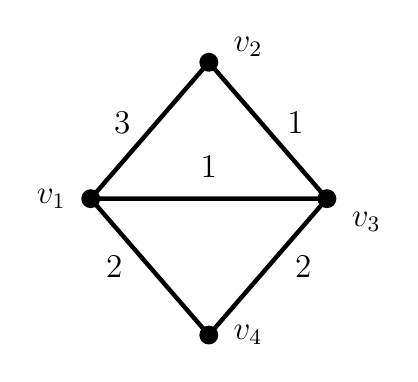
\begin{tikzpicture}[scale=1.00]

\coordinate (p1) at (-1.5, 0.000);
\coordinate (p2) at ( 0.0, 1.732);
\coordinate (p3) at ( 1.5, 0.000);
\coordinate (p4) at ( 0.0,-1.732);
\foreach \x in {1,...,4}{\fill (p\x) circle (0.12);}

\node at ($(p1)+(-0.5, 0.00)$) {\large $v_1$};
\node at ($(p2)+(+0.5, 0.20)$) {\large $v_2$};
\node at ($(p3)+(+0.5,-0.30)$) {\large $v_3$};
\node at ($(p4)+(+0.5, 0.00)$) {\large $v_4$};

\draw[ultra thick] (p1)--(p2)--(p3)--(p4)--(p1)--(p3);
\node at ($(p1)!0.5!(p2)+(-0.35, 0.1)$) {\large $3$};
\node at ($(p1)!0.5!(p4)+(-0.45, 0.0)$) {\large $2$};
\node at ($(p1)!0.5!(p3)+( 0.00, 0.4)$) {\large $1$};
\node at ($(p2)!0.5!(p3)+(+0.35, 0.1)$) {\large $1$};
\node at ($(p4)!0.5!(p3)+(+0.45, 0.0)$) {\large $2$};
\end{tikzpicture}
\end{center}
\caption{An instance $(H,w_H)$ on which the {\greedy} algorithm fails.}
\label{fig:cactus}
\end{figure}
%%%%%%%%%%%%%%%%%%%%%%%%%%%%%%%%%%%%%%%%%



%%%%%%%%%%%%%%%%%%%%%%%%%%%%%%%%%%%%%%%%%%%%%%%%%%%%%%%%%%%%%%%%%%%%%%%%%
%%%%%%%%%%%%%%%%%%%%%%%%%%%%%%%%%%%%%%%%%%%%%%%%%%%%%%%%%%%%%%%%%%%%%%%%%
\section{Parameterized Complexity}
\label{sec:parameterized}
%%%%%%%%%%%%%%%%%%%%%%%%%%%%%%%%%%%%%%%%%%%%%%%%%%%%%%%%%%%%%%%%%%%%%%%%%
In this section, we show that problem {\xxxNTP} is fixed parameter tractable with 
respect to various parameters. 
Note that we showed in \cref{thm:hardness_complete_bipartite,thm:hardness_bandwidth,th:small-weights}, 
that problem {\xxxNTP} is NP-complete, even if either the treewidth or the weights are bounded by a constant. 
If on the other hand both treedwidth and weights are bounded, the following theorem shows that 
the problem can be solved in linear time.

\begin{theorem}
Let $k$ be a bound on both the treewidth of the input graph and on the maximum edge weight.
Problem {\xxxNTP} is fixed parameter tractable with respect to parameter $k$.
\end{theorem}
\begin{proof}
Let $(G, w)$ be an instance of {\xxxNTP}, such that $G = (V, E)$ has treewidth at most $k$, and $w(e) \leq k$ for all edges. Because $G$ has treewidth at most $k$, there exists a vertex $v$ of degree at most $k$. Every edge incident to $v$ has weight at most $k$. Hence the maximum value of a solution is at most $k^2$. For every $T \in \{1,\dots,k^2\}$, we construct a formula $\Phi_T$ in monadic second-order graph logic $\text{MSO}_2$, such that $\Phi_T$ is satisfiable if and only if a schedule of objective value at least $T$ exists. In fact, we introduce binary variables $x_{e,t}$ for $e \in E$ and $t \in \{1,\dots,T\}$. Then the following expression can be formulated in $\text{MSO}_2$:
\begin{align*}
\exists \sigma: E\to\{0,\ldots,&T\} ~~\forall e\in E ~~\forall t\in\{1,\ldots,T\}: \\
& (x_{e,t}=1) \iff \left(\sigma(e) < t \leq \sigma(e) + w(e)\right)\\
& \land \forall t\in\{1,\ldots,T\}: \set{e\in E \mid x_{e,t} = 1} \text{ is a spanning tree.}
\end{align*}
It follows from Courcelle's theorem \cite{courcelle1990monadic}, that for each $T\in\{1,\dots,k^2\}$ the 
satisfiability of $\Phi_T$ can be checked in linear time. This proves the claim.
\end{proof}

\begin{theorem}
\label{th:exact}
On connected graphs $G=(V,E)$, problem {\xxxNTP} can be solved in exponential time $\bigO(|E|^2\cdot|E|!)$.
\end{theorem}
\begin{proof}
Call a schedule $\sigma$ of objective value $T$ \emph{non-dominated}, if none of the graphs 
$G_1^\sigma, \dots, G_T^\sigma$ contain a cycle. 
For any dominated schedule $\sigma$, it is easy to find a non-dominated $\sigma'$ with $\ntp(\sigma')\ge\ntp(\sigma)$. 
(One just schedules some edges at a later moment in time, which is never worse.) 
But observe that a non-dominated schedule is uniquely defined by the order $e_1, \dots, e_k$ 
in which its edges are activated. 
It follows that there are at most $k!$ different non-dominated schedules. 
It is easy to see that the objective value of a single schedule can be evaluated in $\bigO(k^2)$ time. 
\end{proof}

Next, we show that problem {\xxxNTP} is fixed parameter tractable with respect to the size $k$ 
of a feedback edge set. 
As the graph $G=(V,E)$ is undirected and connected, we have $k=|E|-(n-1)$.

\begin{theorem}
\label{thm:FPT_feedback_edge_set}
Problem {\xxxNTP} is fixed parameter tractable with respect to the size $k$ of a feedback edge set. 
The algorithm has a running time of $\bigO((k^2)!k^4n)$. 
\end{theorem}

\begin{proof}
We assume that $G$ consists of a spanning tree $T$ together with $k$ additional edges $e_1,\ldots,e_k$. 
Let $C$ be a cycle in $G$ with at least $2k+2$ edges, if such a cycle exists. 
Let $f_1,\ldots,f_{|C|}$ be the edges of $C$ ordered by weight, that is, $w(f_1) \leq w(f_2) \leq \dots w(f_{|C|})$. 
We claim that any schedule $\sigma$ satisfies $\ntp(\sigma)\le w(f_{2k+2})$. 
Indeed, we may assume that there are exactly $k$ edges in $E$ that satisfy $\sigma(e)\ne0$; 
call these edges $e_1', \dots e'_k$. 
In particular, at least $k+2$ edges in the set $\fromto{f_1}{f_{2k+2}}$ satisfy $\sigma(e)=0$, 
and all of these are inactive during the time slot $[w(f_{2k+2}), w(f_{2k+2}) + 1]$. 
Hence, during this time slot, the cycle $C$ disintegrates into at least $k+2$ components, which need 
to be reconnected by using the edges $e_1', \dots, e'_k$. But this is clearly impossible. 
Hence, $\ntp(\sigma) \leq w(f_{2k+2})$. 
As a consequence, if a cycle $C$ in $G$ has length more than $2k+2$, we can contract the heaviest 
edges until $C$ has exactly $2k+2$ edges, and obtain an equivalent instance.

We now describe how to obtain a kernel of size $\bigO(k^2)$. For each of $i \in \fromto{1}{k}$, let $C_i$ be the unique cycle in $T + e_i$. By the above argument, we can assume that $|C_i| \leq 2k+2$. If $e \in E$ is an arbitrary edge, it is either contained in some $C_i$, or not contained in any cycle. If $e$ is not contained in any cycle, it is very easy to handle when solving problem {\xxxNTP}. Therefore, $\bigcup_{i=1}^k C_i$ is a kernel of size $\bigO(k^2)$. The running time follows from Theorem~\ref{th:exact}.
\end{proof}

The final theorem of this section shows, that problem {\xxxNTP} is tractable on instances, which are in some sense close to the spanning tree packing problem. Here we assume that the graph can have an arbitrary amount of edges, however, almost all edge weights are equal to one. There are at most $k$ edges with weight not equal to one. Additionally, each of these special edges has weight at most $k$. Then, problem {\xxxNTP} is fixed parameter tractable with respect to $k$.

\begin{theorem}
Let $(G,w)$ be an instance of {\xxxNTP} on $n$ vertices and $m$ edges, so that $m-k$ edges have weight~$1$ and the remaining $k$ edges have weight at most $k$. 
Then an optimal solution can be found in $\bigO(k^{2k}m^3)$ time.
\end{theorem}

\begin{proof}
Let $E' := \set{e \in E(G) : w(e) \neq 1}$. (By assumption, $w(e) \leq k$ for all $e \in E'$). If $\sigma$ is a schedule of value $T$ for $(G, w)$,  let $D_\sigma := \set{t \in \fromto{1}{T} : E_t^\sigma \cap E' \neq \emptyset}$ describe the set of time slots $[t-1, t]$ during which some edge of $E'$ is active. Note that  if $t \not\in D_\sigma$, then $G_t = (V, E_t)$ is a connected graph in which all edges $e \in E_t$ have weight 1. We can consider the alternate schedule $\pi$, where the edge set $E_t$ gets scheduled in the last time slot $[T-1, T]$ instead of the $t$-th time slot, and all edges activated during $[t, T]$ are activated one time unit sooner instead. Formally, schedule $\pi$ is such that
\[(G^\pi_1,\dots, G^\pi_T) = (G^\sigma_1, \dots G^\sigma_{t-1}, G^\sigma_{t+1}, \dots, G^\sigma_T, G^\sigma_t) \]

Observe that $\pi$ is also a schedule of objective value $T$. We conclude that there always exists an optimal schedule $\sigma$ such that $D_\sigma \subseteq \fromto{1}{k^2}$. It is also not  hard to see that we can additionally require that each of $G_1, \dots, G_T$ is acyclic.

Therefore, the following is an algorithm to solve problem {\xxxNTP}: Iterate over all possible $k^{2k}$ choices of $(\sigma(e))_{e \in E'} \in \fromto{1}{k^2}^k$. For each fixed choice, the only edges left to schedule are edges of weight one. This can be done optimally the following way: Let $E_i := \set{e \in E' : \sigma(e) = i}$ for $i \in \fromto{1}{k^2}$. If some $E_i$ has a cycle, we can immediately skip to the next choice of $(\sigma(e))_{e \in E'}$. Otherwise, consider the matroid $\mathcal{F}_i := \set{F \subseteq E(G)-E_i : E_i \cup F \text{ is acyclic}}$. We extend the definition of $\mathcal{F}_i$ to $i > k^2$ by setting $E_i := \emptyset$ in this case. The matroid $\mathcal{F}_i$ is isomorphic to the graphic matroid of $G$ after contracting each connected component of $E_i$ to a single vertex. Now we can run
 Edmond's Matroid Partitioning algorithm \cite{edmonds1965minimum} to determine the maximal $T' \in \N_0$ such that $E(G)-E'$ contains disjoint sets $F_1, \dots, F_{T'}$ such that $F_i$ is a base of $\mathcal{F}_i$ for all $i \in \fromto{1}{T'}$ (i.e.\ we solve the problem of packing as many bases as possible into a matroid). Edmond's Matroid Partitioning algorithm runs in $\bigO(
m^3)$ time. Hence the claim is proven.
\end{proof}


%%%%%%%%%%%%%%%%%%%%%%%%%%%%%%%%%%%%%%%%%%%%%%%%%%%%%%%%%%%%%%%%%%%%%%%%%
%%%%%%%%%%%%%%%%%%%%%%%%%%%%%%%%%%%%%%%%%%%%%%%%%%%%%%%%%%%%%%%%%%%%%%%%%
\section{Conclusion}
\label{sec:conclusion}
%%%%%%%%%%%%%%%%%%%%%%%%%%%%%%%%%%%%%%%%%%%%%%%%%%%%%%%%%%%%%%%%%%%%%%%%%

\begin{itemize}
\item  We showed that {\xxxNTP} can be approximated by a factor $n-1$, but can not be approximated 
by a factor better than $7/6$ even if $w(e) \in \fromto{1}{6}$. 
We were not able to find approximation algorithms for {\xxxNTP} with $\bigO(1)$ approximation ratios. 
\textbf{Conjecture:} In the general case, there exists no $\bigO(1)$-approximation algorithm for {\xxxNTP}.
\item Is the case where $w(e) \in \set{1, 2}$ for all edges polynomially solvable?
\item We showed it can  be decided in poly-time, whether $\ntp(G, w) \geq 3$, but it is NP-hard to decide, whether $\ntp(G, w) \geq 7$. 
\item FTP-results coupd be obtained.
\end{itemize}


\subsubsection*{Acknowledgements.}

Stefan Lendl and Lasse Wulf acknowledge the support of the Austrian Science Fund (FWF): W1230.
Gerhard Woeginger acknowledges support by the DFG RTG 2236 ``UnRAVeL''.

%
% ---- Bibliography ----
%
% BibTeX users should specify bibliography style 'splncs04'.
% References will then be sorted and formatted in the correct style.

\bibliographystyle{splncs04}
\bibliography{literature}


%%%%%%%%%%%%%%%%%%%%%%%%%%%%%%%%%%%%%%%%%%%%%%%%%%%%%%%%%%%%%%%%%%%%%%%%%
%%%%%%%%%%%%%%%%%%%%%%%%%%%%%%%%%%%%%%%%%%%%%%%%%%%%%%%%%%%%%%%%%%%%%%%%%
\appendix
\section{Avoiding edges of weight 7 in \cref{th:small-weights}}
\label{appendix:small-weights-improvement}
We proved in \cref{th:small-weights} that it is NP-hard to decide whether there exists a schedule of objective value 7 for problem {\xxxNTP}. The edge weights in the involved instance were from the set $\fromto{1}{7}$. We can make a small improvement, so that edges of weight 7 are avoided. Note that the only edges of weight 7 occured in the gadgets of type $L$. \cref{fig_hamilton_cycle_improved} shows a modified version of the gadget, which avoids edges of weight 7. One easily sees that \cref{lemma:gadgets_properties} still holds for the modified version of gadget $L$. The rest of the proof is exactly the same as beforehand.
\begin{figure}[htpb]
\centering
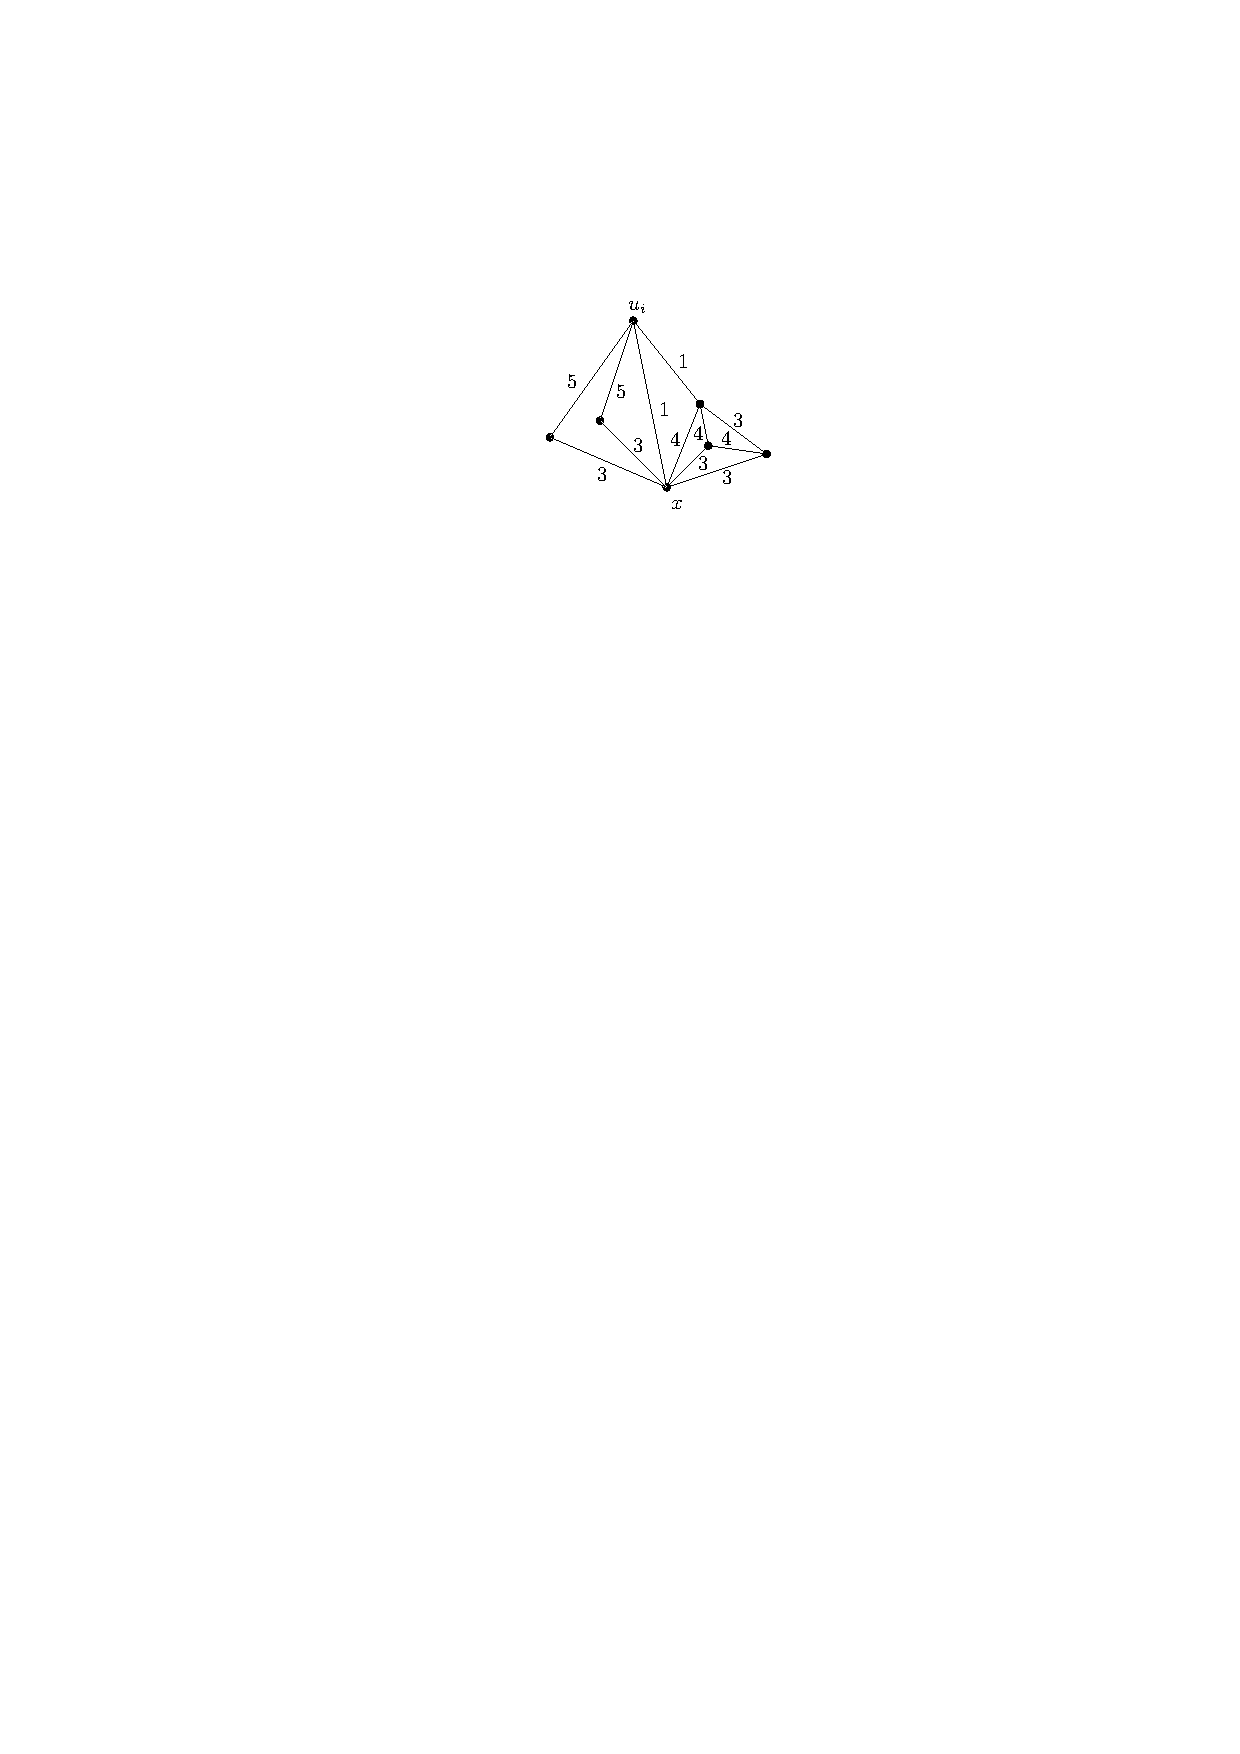
\includegraphics[scale=1]{img/act-hamilton-cycle-b}
\caption{The improved version of a gadget of type $L$ avoids edges of weight 7.}
\label{fig_hamilton_cycle_improved}
\end{figure}

%\label{appendix:hamilton_prime}
%\hamiltonPrime*
%
%\begin{proof}
%It is known that the Hamilton cycle problem is NP-complete for bipartite, 3-regular graphs \cite{hamilton3regularBip}. So let $G = (V, E)$ be a bipartite, 3-regular graph. We construct in polynomial time a graph $H$ and an edge $\set{u,z}$, such that the described propeprties for $(H, \set{u,z})$ hold, and such that $H$ has a Hamilton cycle if and only if $G$ has a Hamilton cycle. If we can show this, we are done.
%
%The reduction is shown in \cref{fig_hamilton_cycle_lemma}. Formally, fix some vertex $x \in V$. Let $G_1$ and $G_2$ be two copies of $G$. For each vertex $v \in V-\set{x}$, take a copy $A_v$ of $K_{4,4}$, remove some edge $\set{u_1, u_2}$ from $A_v$, and add edges $\set{v_1,u_1}$ and $\set{u_2,v_2}$, where $v_i$ is the copy of $v$ in $G_i$, $i = 1,2$. Finally, take two copies $A_x$ and $A'_x$ of $K_{4,4}$, remove an edge $\set{u_1,u_2}$ from $A_x$ and an edge $\set{u'_1,u'_2}$ from $A'_x$, add edges $\set{x_1,u_1}$, $\set{u_2,u'_1}$, $\set{u'_2,x_2}$, and let the special edge be given by $\set{u, z}$ with $u := u_2$, and $z := u'_1$. Clearly, $H$ is bipartite and 4-regular.
%
%Let (iv) be the property that $G$ has a Hamilton cycle. We show that (i) -- (iv) are equivalent, thus proving the theorem. So assume (i) holds. It is easy to see that any Hamilton cyle in $H$ uses $\set{u,z}$, so (ii) holds. Assume (ii) holds, (iii) follows immediately. Assume (iii) holds, i.e.\ there is a Hamilton path $(w_1, \dots, w_n)$ starting at $u$. Note that if $w_2 = z$, then $w_n$ is in $A_x$. On the other hand, if $w_2$ is in $A_x$, then $w_n$ is in $A'_x$. In both cases, we can slightly modify $P$ to obtain a Hamilton cycle. Therefore, (i) holds. Finally, we show that (i) and (iv) are equivalent. If $G$ has a Hamilton cycle, we can modify it to obtain a Hamilton cycle of $H$, by switching between $G_1$ and $G_2$ after every edge of the original Hamilton cycle and inserting a Hamilton path through the copies of $K_{4,4}$ (note that $G$ has an even number of vertices, as it is 3-regular). On the other hand, if $H$ has a Hamilton cycle, it necessarily switches between $G_1$ and $G_2$ after every of its edges in $G_1$ or $G_2$, so $G$ has a Hamilton cycle.
%\end{proof}
%\begin{figure}[htpb]
%\centering
%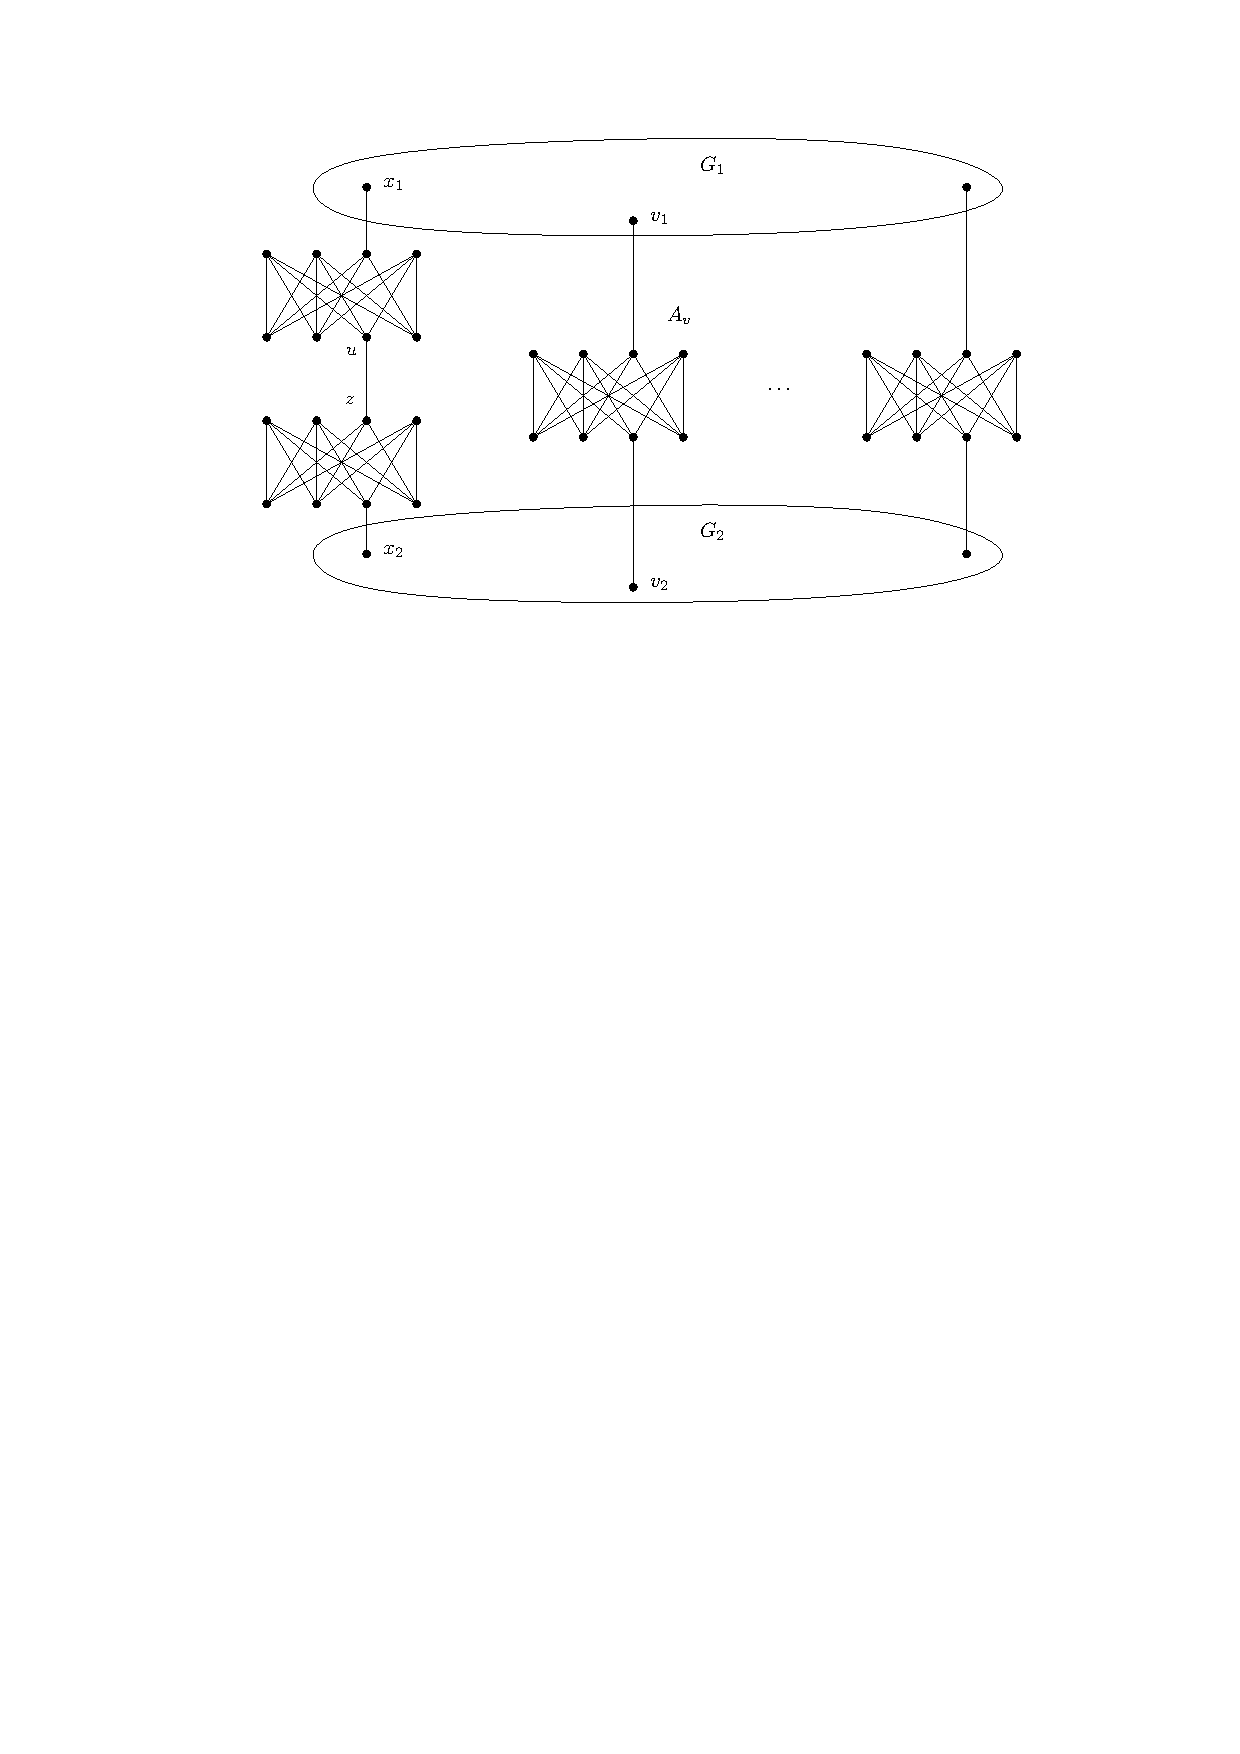
\includegraphics[scale=0.92]{img/hamilton-prime}
%\caption{Construction used in the proof of \cref{hamilton_cycle_lemma}.}
%\label{fig_hamilton_cycle_lemma}
%\end{figure}

\end{document}
